\documentclass{beamer}

\usetheme{Madrid}
\usepackage[utf8]{inputenc}
\usepackage[makeroom]{cancel}
\usepackage{amsmath}
\usepackage{manfnt}
\usepackage{graphicx}
\usepackage[dvipsnames]{xcolor}
\definecolor{dgreen}{rgb}{0.,0.6,0.}
\usepackage{amssymb}
\usepackage{pifont}

\graphicspath{ {figures/} }

\renewcommand{\vec}[1]{\boldsymbol{#1}}
\newcommand{\vecg}[1]{\mathbold{#1}}
\newcommand{\matr}[1]{\mathbf{#1}}
\newcommand{\cmark}{\ding{51}}%
\newcommand{\xmark}{\ding{55}}%

\date{xy/03/2017}

\title[Hybrid Impedance Control]{Hybrid Impedance Control of a Kuka LWR 4+}
\subtitle{Corso di Laurea Magistrale in Ingegneria Robotica ed Automazione \\
  Controllo dei Robot}
\author{Nicola Piga, Giulio Romualdi}
\institute[]{Università di Pisa}

\begin{document}
\beamertemplatenavigationsymbolsempty

\begin{frame}
  \maketitle
  \centering
  \begin{columns}
    \begin{column}{0.4\columnwidth}
    \end{column}
    \begin{column}{0.265\columnwidth}
      \centering
      
\includegraphics[width=20mm]{cherubino}
    \end{column}
    \begin{column}{0.6\columnwidth}
      \vskip.1in
      \hskip.3in
      Supervisors:\\
      \hskip.3in
      Prof. Antonio Bicchi\\
      \hskip.3in
      Ing. Manuel Bonilla\\
    \end{column}
  \end{columns}
\end{frame}

\section{Description of the task}\label{sec:task_description}
This section serves as a preliminary one for the rest of the report. The main task
of interest is briefly recalled and several frames of reference are introduced within
the typical setup in which the task is performed. These frames of reference, along
with some notations and conventions, will be useful to easily identify the quantities
that belong to the state of the controllers developed in the next sections of this report.

\subsection{Typical set-up}
The typical setup, as shown in figure \ref{fig:frames}, consists of a $7$-joints KUKA LWR $4$+
anthropomorphic manipulator equipped with an hand-like end-effector, a table and an object that the hand is not
able to grasp using its primitives.
\begin{figure}[h]
  \centering
  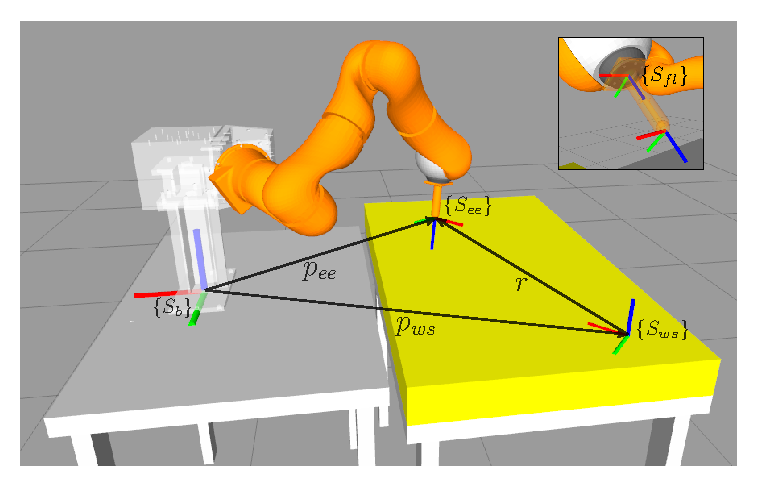
\includegraphics[scale=0.9]{frames.pdf}
  \caption{Typical set-up with reference frames \label{fig:frames}}
\end{figure}
Then the task to be performed consists in dragging the object on the table, hence exploiting
the environonmental constraints offered by the surface of the table, until the object sticks
out of the border of the table and a standard grasp is feasible. Also the dragging phase should
be accomplished without damaging the object or the hand because of too high contact forces between
the object and the surface of the table or between the object and the hand.
For this reason the manipulator is equipped with a force/torque sensor which is rigidely attached
to the last link of the robot and measures forces and torques exchanged at the wrist of the robot.
The hand is connected to the sensor using a mounting plate and a clamp.

\subsection{Division of the task in phases}\label{sec:task_division}
The dragging phase described above can be considered as the \emph{final} part of a more
complex task which should be divided, at least, in three parts:
\begin{itemize}
\item[-] approaching phase in which the robot moves the hand near the object of interest;
\item[-] contact phase in which the contact between the hand and the object takes place;
\item[-] dragging phase.
\end{itemize}

In the rest of the this report more attention is given to the dragging phase since it is the phase
where the hybrid force position strategy is used. As regards the contact phase the experimental results,
presented in the last section, show that it can be achieved using the same controller used in the dragging
phase. The approaching phase is also described in a separate section.

\subsection{Frames of reference}\label{sec:frames}
In order to develop a control system that is able to regulate the position of the object
and the force exerted on it, i.e. an hybrid force position control system, while the hand
is dragging the object on the table
a natural choice for a basis in which express the commanded positions and forces is that of
an inertial reference frame with the origin $W$ on a point of the table and the $x$ and $y$ axes parallel to the surface
of the table
\[
\{S_{ws}\} = \{W; x_{ws}, y_{ws}, z_{ws} \}
\]
where \emph{ws} stands for ``workspace'' since the table represents the intended workspace
for the robot. This choice allows to specify the commanded position as 2-dimensional vector
with components along the directions $\hat{\vec{i}}_{ws}$ and $\hat{\vec{j}}_{ws}$ and the
commanded force as a positive scalar along the direction $-\hat{\vec{k}}_{ws}$.
A quantity related to this reference frame is the vector $\vec{r}$ going from the origin $W$
to the center of the palm of the hand.
\par
A second reference frame to be introduced is an inertial frame fixed to the main base of the robot
\[
\{S_b\} = \{B; x_b, y_b, z_b \}
\]
Similarly to $\vec{r}$ the vector $\vec{p}_{ee}$ goes from $B$ to the center of the palm of the hand.
It should be noted that frames $\{S_{ws}\}$ and $\{S_b\}$ have no relative orientation and that
the vector $\vec{p}_{ws}$ going from $B$ to $W$ is constant. As a consequence the vector $\vec{r}(t)$
can be express as
\[
\vec{r}(t) = \vec{p}_{ee}(t) - \vec{p}_{ws}
\]
where $\vec{p}_{ws}$ is known and $\vec{p}_{ee}(t)$ is given by forward kinematics
numerical routines such as those offered by the library KDL used in this project.
The frame $\{S_b\}$ is also the frame in which the library KDL expresses quantities
like the vector $\vec{p}_{ee}$, the Jacobians and their derivatives.
\par
Other reference of frames of interest are those fixed to the end-effector
\[
\begin{split}
  &\{S_{fl}\} = \{F; x_{fl}, y_{fl}, z_{fl} \}\\
  &\{S_{ee}\} = \{E; x_{ee}, y_{ee}, z_{ee} \}
\end{split}
\]
where $F$ corresponds to the center of the wrist of the robot and $E$ is in the center
of the palm of the hand. These frames, that have no relative orientation,  are of interest
mainly because the signal produced by the force/torque sensor are expressed in these frames.

\subsection{Notation and convention}
In the rest of this report the following notation will be used to express any quantity $X$ encountered:
\[
\prescript{b}{}{X}_p
\]
where $b$ specify the reference frame $\{S_b\}$ in which $X$ is expressed and, whenever
$X$ is a wrench or a Jacobian $J$ such that $X\vec{\dot{q}}$ is a twist, $p$ specify the
reference point of that wrench or that twist. In case $X$ is an analytical Jacobian or $X$ is a vector
containing \emph{also} angular displacement or angular rates it should be clear that the specification
of a basis has no meaning and it applies only to a part of the vector.
\par
This notation is very general and sometimes the prescript $b$ and/or the subscript $p$ will
be missing when they are clear from the context.

\newpage


\section{Hybrid impedance control}

\begin{frame}{Hybrid impedance control [Anderson, Spong, 1988]}
  The Hybrid Impedance Control approach features \alert{a more general concept of
  impedance} than that used in typical PD position controllers with tuned
  apparent impedances of the form
  \[
  (\ddot{\vec{x}}^{des} - \ddot{\vec{x}}) + K_{damping} (\dot{\vec{x}}^{des} - \dot{\vec{x}})
  + K_{stifness}(\vec{x}^{des} - \vec{x}) = \vec{F}
  \]
  \par
  It allows to synthesize for each DoF of the manipualator both a position or a \alert{direct
    force} controller by matching a given ``environment impedance'' with the appropriate
  ``manipulator impedance''
\end{frame}

\begin{frame}{HIC - Type of impedances}
  \centering
  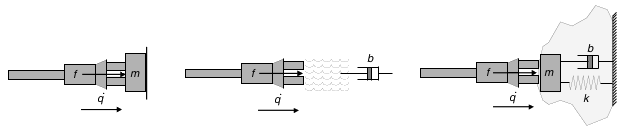
\includegraphics[scale=0.65]{type_of_impedances.png}
  \begin{itemize}
  \item[-] for each cartesian DoF the manipulator and the environment can be described using impedances $Z_m$ and $Z_e$
  \item[-] the environment is defined to be any element connected
    to or contacting the robot anywhere \alert{past the wrist} force sensor
  \item[-] $Z(\omega) = R(\omega) + j X(\omega)$
  \item[-] type of impedances
    \begin{itemize}
    \item[] inertial iff $|Z(0)| = 0$
    \item[] resistive iff $|Z(0)| = c \in (0, \infty)$
    \item[] capacitive iff $|Z(0)| \rightarrow \infty$
    \end{itemize}
  \end{itemize}
\end{frame}

\begin{frame}{HIC - Duality principle and equivalence to circuit theory}
  \begin{block}{Duality principle}
    The manipulator should be controlled to respond as the dual of the environment
  \end{block}

  This principle is most easily described in terms of Norton and Thèvenin equivalents
  \begin{itemize}
  \item[-] an inertial environment is represented using a Thèvenin equivalent
  \item[-] a capacitive environment is represented using a Norton equivalent
  \item[-] a resistive environment is represented using either a Thèvenin or a Norton equivalent
  \end{itemize}
\end{frame}

\begin{frame}[shrink=10]{HIC - Duality principle for position control}
  Manipulator impedance chosen as the dual of the environment impedance in order to obtain zero
  steady state error to a step input
  \vskip0.1in
  \begin{columns}
    \begin{column}{0.5\columnwidth}
      \begin{flalign*}
        v = \frac{Z_m(s)}{Z_m(s) + Z_e(s)}v_{des} - \frac{F_{env}}{Z_e + Z_m}
      \end{flalign*}
    \end{column}
    \begin{column}{0.5\columnwidth}
      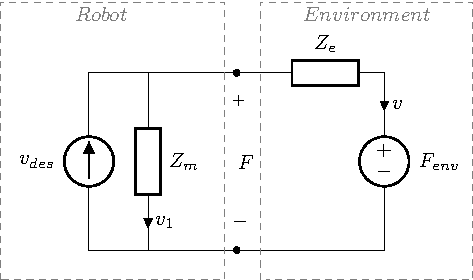
\includegraphics[width=\columnwidth]{position_control_model}
    \end{column}
  \end{columns}
  \par
  \[
  e_{ss} \Big|_{F_{env} \equiv 0} = \lim_{s \to 0}(v - v_{des}) = \frac{-Z_e(0)}{Z_m(0) + Z_e(0)} = 0
  \]
  \[
  \alert{\text{as long as } Z_m(0) \neq 0 \text{ and } Z_e(0) = 0}
  \]
  \par

  \begin{exampleblock}{Rule of thumb}
    inertial environments are position controlled with a noninertial manipulator impedance
    (the actual value of $Z_e(0)$ \alert{should not be known})
  \end{exampleblock}
\end{frame}

\begin{frame}[shrink=30]{HIC - Position controlled subsystem}
  The electrical circuit \alert{can be seen as a control feedback scheme where $a$ is the \alert outer loop
  acceleration} corresponding to the desired velocity $v_{des}$
  \begin{columns}
    \begin{column}{0.4\textwidth}
      \begin{align*}
        &v_{des} = v + v_1\\
        &v_1 = \frac{F}{Z_m}\\ 
        &F = Z_e v + F_{env}\\
        &a = \dot{v} = \frac{\mathrm{d}}{\mathrm{d}t} \left(v_{des} - \frac{F}{Z_m} \right)\\
        &Z_m = M s + \tilde{Z}_m\\
      \end{align*}
    \end{column}
    \begin{column}{0.5\textwidth}
      \centering
      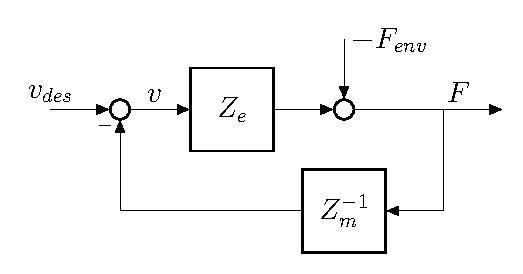
\includegraphics[scale=0.8]{position_control_feedback}
    \end{column}
  \end{columns}
  The acceleration can be written \alert{without derivatives}
  \begin{align*}
    &a = \frac{\mathrm{d}}{\mathrm{d}t} \left(v_{des} - \frac{F}{Ms + \tilde{Z}_m} \right) = \dot{v}_{des} - \frac{Fs}{Ms + \tilde{Z}_{m}} = \dot{v}_{des} - s v_1 \\
    &F = v_1 (Ms + \tilde{Z}_m) \quad v_1 = \frac{F - (v_{des} - v)\tilde{Z}_m}{Ms}\\
    &a = \dot{v}_{des} - s v_1 = \dot{v}_{des} - \cancel{s} \left( \frac{F - (v_{des} - v)\tilde{Z}_m}{M\cancel{s}} \right) = \dot{v}_{des} + \frac{(v_{des} - v)\tilde{Z}_m}{M} - \frac{F}{M}
  \end{align*}
\end{frame}

\begin{frame}[shrink=10]{HIC - Duality principle for force control}
  Manipulator impedance chosen as the dual of the environment impedance in order to obtain zero
  steady state error to a step input
  \vskip0.1in
  \begin{columns}
    \begin{column}{0.5\columnwidth}
      \begin{flalign*}
        F = \frac{Z_e(s)}{Z_m(s) + Z_e(s)}F_{des} + \frac{Z_e Z_m}{Z_m + Z_e} V_{env}
      \end{flalign*}
    \end{column}
    \begin{column}{0.45\columnwidth}
      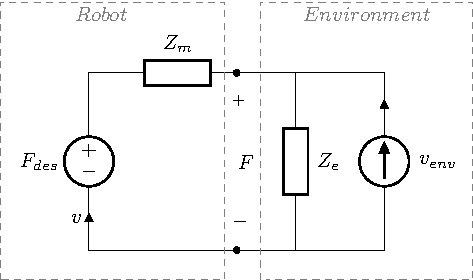
\includegraphics[width=\columnwidth]{force_control_model}
    \end{column}
  \end{columns}
  \[
  e_{ss} \Big|_{v_{env} \equiv 0} = \lim_{s \to 0}(F - F_{des}) = \frac{-Z_m(0)}{Z_m(0) + Z_e(0)} = 0 
  \]
  \[
  \alert{\text{as long as } Z_m(0) < \infty \text{ and } Z_e(0) \rightarrow \infty}
  \]
  \begin{exampleblock}{Rule of thumb}
    capacitive environments are force controlled with a noncapacitive manipulator impedance
    (the actual value of $Z_e(0)$ \alert{should not be known})
  \end{exampleblock}
\end{frame}

\begin{frame}[shrink=30]{HIC - Force controlled subsystem}
  The electrical circuit \alert{can be seen as a control feedback scheme where $a$ is the outer loop
  acceleration} of the DoF corresponding to the desired force $F_{des}$
  \begin{columns}
    \begin{column}{0.4\textwidth}
      \begin{align*}
        &F = F_{des} + Z_m v\\
        &v = \frac{F - F_{des}}{Z_m}\\
        &F = Z_e(v + v_{env})\\
        &a = \dot{v} = \frac{\mathrm{d}}{\mathrm{d}t} \left(\frac{F - F_{des}}{Z_m} \right)\\
        &Z_m = M s + \tilde{Z}_m\\
      \end{align*}
    \end{column}
    \begin{column}{0.5\textwidth}
      \centering
      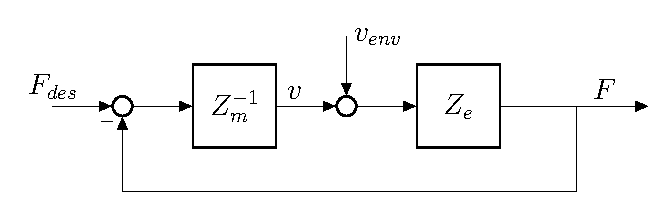
\includegraphics[scale=0.8]{force_control_feedback}
    \end{column}
  \end{columns}
  The acceleration can be written \alert{without derivatives}
  \begin{align*}
    &a = \frac{\mathrm{d}}{\mathrm{d}t} \left(\frac{F - F_{des}}{Ms + \tilde{Z}_m} \right) = \left(\frac{s(F - F_{des})}{Ms + \tilde{Z}_m} \right)\\
    &vMs + v \tilde{Z}_m = F - F_{des}\\
    &v = \frac{1}{Ms} (F - F_{des} - v \tilde{Z}_m )\\
    &a = \dot{v} = \frac{\cancel{s}}{M\cancel{s}} (F - F_{des}) - \frac{\cancel{s}}{M\cancel{s}}( \tilde{Z}_m v) = \frac{1}{M} (F - F_{des}) - \frac{1}{M}( \tilde{Z}_m v)
  \end{align*}
\end{frame}

\section{HIC based control architecture}

\begin{frame}{References frames}
  Before delving into an HIC based controller let us introduce some useful reference frames and notation
  \begin{columns}
    \begin{column}{0.7\columnwidth}
      \begin{center}
        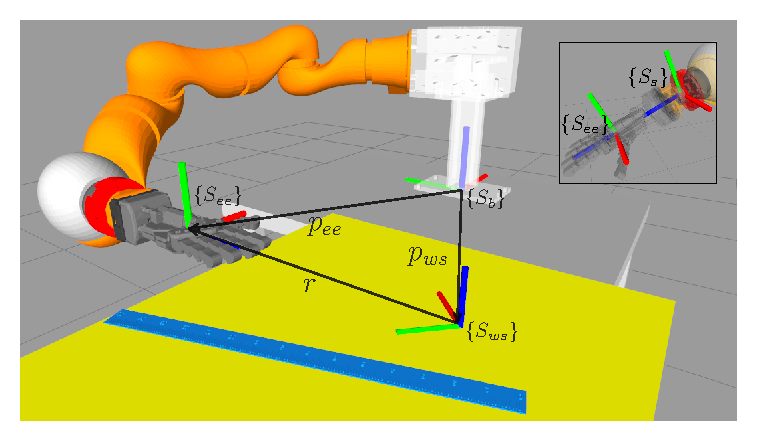
\includegraphics[width=\columnwidth]{frames_new}
      \end{center}
    \end{column}
    \begin{column}{0.3\columnwidth}
      \begin{itemize}
      \item[$b$:] base 
      \item[$s$:] sensor 
      \item[$ee$:] end-effector (hand) 
      \item[$ws$:] work-space (table) 
      \end{itemize}
    \end{column}
  \end{columns}
  \vskip-1em
  \begin{columns}
    \begin{column}{0.5\columnwidth}
      \begin{flalign*}
        &\{S_{b}\} = \{B; x_b, y_b, z_b \}\\
        &\{S_{s}\} = \{S; x_{s}, y_{s}, z_{s} \}
      \end{flalign*}
    \end{column}
    \begin{column}{0.5\columnwidth}
      \begin{flalign*}
        &\{S_{ee}\} = \{E; x_{ee}, y_{ee}, z_{ee} \}\\
        &\{S_{ws}\} = \{W; x_{ws}, y_{ws}, z_{ws} \}
      \end{flalign*}
    \end{column}
  \end{columns}
\end{frame}

\begin{frame}{Notation}
  \begin{block}{Space state vector definition}
    A natural choice for a basis in which the commanded positions and forces are \alert{expressed is $ws$}
    \[
    \prescript{ws}{}{\vec{x}} = 
    \begin{bmatrix}
      \prescript{ws}{}{r}_x & \prescript{ws}{}{r}_y & \prescript{ws}{}{r}_z & \psi & \theta & \phi
    \end{bmatrix}^T
    \]
    \[
    \prescript{ws}{}{R}_{ee} = R_{ZYZ}(\psi, \theta, \phi) = R_{ZYZ}(\vec{\Phi})
    \]
  \end{block}
  \begin{block}{Convention}
    Convention used for any quantity $X$ encountered, $\prescript{b}{}{X}_p$
    \begin{itemize}
      \item[-] $\prescript{b}{}{.}$ reference frame
      \item[-] $._p$ reference point (for wrench and Jacobian only)
    \end{itemize}
  \end{block}
\end{frame}

\begin{frame}{Control aims}
  \alert{Suppose} that the second derivative of the state can be chosen arbitrarily
  \[
  \prescript{ws}{}{\ddot{\vec{x}}} = \vec{a}_{cmd}
  \]
  Find $\vec{a}_{cmd}$ using HIC such that
  \begin{itemize}
  \item[-]$r_x$, $r_y$ and $\vec{\Phi}$ are rigidly controlled i.e.
    \begin{itemize}
    \item[i.] $\ddot{e}_{x} + B_x \dot{e}_x + K_x e_x = 0 \quad \quad  e_x(t) =   \prescript{ws}{} r_{x,des}(t) - \prescript{ws}{} r_{x}(t)$
    \item[ii.] $\ddot{e}_{y} + B_y \dot{e}_y + K_y e_y = 0 \quad \quad e_y(t) =   \prescript{ws}{} r_{y,des}(t) - \prescript{ws}{} r_{y}(t)$
    \item[iii.] $\ddot{\vec{e}}_{\Phi} + B_{\Phi} \dot{\vec{e}}_{\Phi} + K_{\Phi} \vec{e}_{\Phi} = \vec{0} \quad \quad \vec{e}_{\Phi}(t) = \vec{\Phi}_{des}(t) - \vec{\Phi}(t)$
    \end{itemize}
  \item[-]the DoF along $z_{ws}$ is force controlled i.e.
    \begin{itemize}
    \item[i.] $e_z \xrightarrow[t \to \infty] {} 0 \quad \quad e_{z}(t) = \prescript{ws}{} F_{z,des}(t) - \prescript{ws}{} F_{z}(t)$
    \end{itemize}
  \end{itemize}
  where $\prescript{ws}{} F_{z}(t)$ is the force exerted by the hand to the object expressed in $ws$
\end{frame}

\begin{frame}[shrink=30]{Resulting HIC based controller}
  \begin{block}{Position ($\prescript{ws}{}{r}_x$, ${}^{ws}r_y$)}
  \begin{itemize}
  \item[-] inertial environment supposed, i.e., manipulator moving a payload along given axis
  \item[-] $Z_{m,p} = M_p s + \tilde{Z}_{m,p} = M_p s + B_p + \frac{K_p}{s} = s + B_p + \frac{K_p}{s} $
  \end{itemize}
  \[
  \begin{split}
    & \prescript{ws}{}{a}_{cmd,x} = \ddot{r}_{x,des} + B_x (\dot{r}_{x,des} - \dot{r}_x) + K_x (r_{x,des} - r_x) - F_x \\
    & \prescript{ws}{}{a}_{cmd,y} = \ddot{r}_{y,des} + B_y (\dot{r}_{y,des} - \dot{r}_y) + K_y (r_{y,des} - r_y) - F_y
    \end{split}
  \]
  \end{block}
  \begin{block}{Attitude ($\psi$, $\theta$, $\phi$)}
    \begin{itemize}
    \item[-] inertial environment supposed, i.e., manipulator rotating a payload about given axis
    \item[-] $Z_{m,a} = M_a s + \tilde{Z}_{m,a} = M_a s + B_a + \frac{K_a}{s} = s + B_a + \frac{K_a}{s}$
    \end{itemize}
    \[ 
    \prescript{ws}{}{\vec{a}}_{cmd,\Phi} = \ddot{\vec{\Phi}}_{des} + B_{\Phi} (\dot{\vec{\Phi}}_{des} - \dot{\vec{\Phi}}) + K_{\Phi} (\vec{\Phi}_{des} - \vec{\Phi})
    \]
  \end{block}
  \begin{block}{Force (${}^{ws}F_z$)}
    \begin{itemize}
    \item[-] capacitive environment supposed
    \item[-] $Z_{m,f} = M_f s + \tilde{Z}_{m,f} = M_f s + \tilde{B}_f = \frac{s}{K_f} + \frac{B_f}{K_f}$
    \end{itemize}
    \[
    \prescript{ws}{}{a}_{cmd,z} = - B_f \dot{r}_z + K_f(F_{z,des} - F_z)
    \]  
  \end{block}
\end{frame}

\begin{frame}
  \centering
  \frametitle{Description of reference frames}
  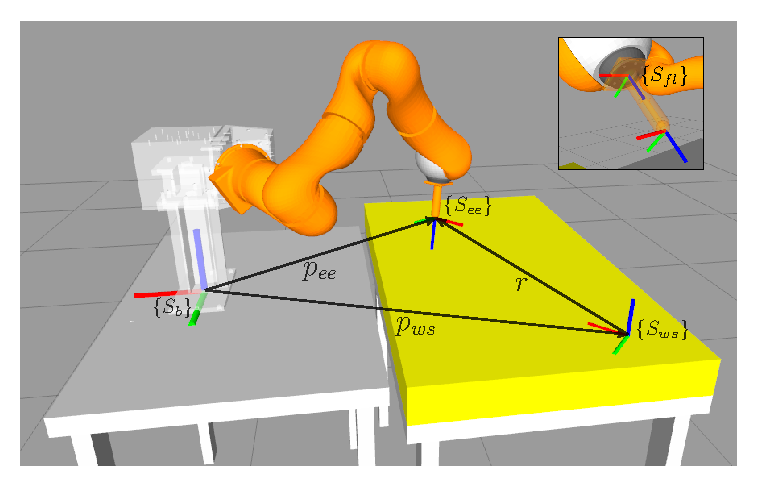
\includegraphics[scale=0.8]{frames}
  \begin{columns}
    \begin{column}{0.45\textwidth}
      \begin{itemize}
      \item[]$\{S_b\} = \{B; x_b, y_b, z_b \}$
      \item[]$\{S_{fl}\} = \{F; x_{fl}, y_{fl}, z_{fl} \}$
      \end{itemize}
    \end{column}
    \begin{column}{0.45\textwidth}
      \begin{itemize}
      \item[]$\{S_{ee}\} = \{E; x_{ee}, y_{ee}, z_{ee} \}$
      \item[]$\{S_{ws}\} = \{W; x_{ws}, y_{ws}, z_{ws} \}$
      \end{itemize}
    \end{column}
  \end{columns}
\end{frame}

\begin{frame}[shrink=15]
  \frametitle{Equations of motion}
  \begin{block}{}
    \begin{equation*}
      B(\vec{q}) \ddot{\vec{q}} + C(\vec{q}, \dot{\vec{q}}) \dot{\vec{q}} + \cancel{\vec{G}(\vec{q})} = \vec{\tau} - {}^{b}J^{T}_{F} {}^b\vec{w}_{F} 
      \longrightarrow {}^{ws}\ddot{\vec{x}} = \vec{a}
    \end{equation*}
    \begin{equation*}
      \vec{q} = 
      \begin{bmatrix}
        q_1 & q_2 & q_3 & q_4 & q_5 & q_6 & q_7
      \end{bmatrix}^T
      \quad
          {}^{ws}\vec{x} = 
          \begin{bmatrix}
            r_x & r_y & r_z & \psi & \theta & \phi
          \end{bmatrix}^T
    \end{equation*}
    \begin{equation*}
      {}^{ws}R_{ee} = R_{ZYX}(\psi, \theta, \phi) = R_{ZYX}(\vec{\Phi})
    \end{equation*}
  \end{block}

  \vskip-1em
  \begin{columns}[t]
    \begin{column}{0.4\textwidth}
      \begin{itemize}
      \item<2->[] Joint Space description
      \item<2->[] $\vec{\tau} = C \dot{\vec{q}} + {}^{b}J^{T}_{F} ({}^b\vec{\gamma} + {}^b\vec{w}_{F})$
      \item<3->[] $\ddot{\vec{q}} = B^{-1} ({}^{b}J^{T}_{F}) {}^b\vec{\gamma}$
      \end{itemize}
    \end{column}
    \begin{column}{0.8\textwidth}
      \begin{itemize}
      \item<4->[] HIC requires operational space description
      \item<4->[] ${}^{ws} \ddot{\vec{x}} = {}^{ws} J_{A,E} \ddot{\vec{q}} + {}^{ws} \dot{J_{A,E}} \dot{\vec{q}}$
      \item<5->[] ${}^{ws} J_{A,E} = 
        \left[
          \begin{smallmatrix}
            I & 0 \\
            0 & T^{-1}(\vec{\Phi})
          \end{smallmatrix}
          \right]$
        ${}^{ws} J_{E} \quad {}^{ws}\vec{\omega} = T(\vec{\Phi}) \vec{\dot{\Phi}}$\\
        $\mathrm{det}(T) = -\cos(\theta) \neq 0$\\
        ${}^{ws} \dot{J_{A,E}} = 
        \left[
          \begin{smallmatrix}
            0 & 0 \\
            0 & -T^{-1} \dot{T} T^{-1}
          \end{smallmatrix}
          \right]
             {}^{ws} J_{E} + 
             \left[
               \begin{smallmatrix}
                 I & 0 \\
                 0 & T^{-1}
               \end{smallmatrix}
               \right]
                  {}^{ws} \dot{J}_{E}$
      \end{itemize}
    \end{column}
  \end{columns}
  \begin{columns}
    \begin{column}{2\textwidth}
      \begin{itemize}
      \item<6->[]Substitute $\ddot{\vec{q}}$ in the operational space description
      \item<6->[]${}^{ws} \ddot{\vec{x}} = \underbrace{{}^{ws} J_{A,E} B^{-1} ({}^b J_{F}^T)}_{B_A^{-1}} {}^b \vec{\gamma} + {}^{ws} \ddot{J_{A,E}} \dot{\vec{q}}$
      \item<7->[]$B_A {}^{ws} \ddot{\vec{x}} =  \vec{\gamma} +  B_A  {}^{ws} \dot{J_{A,E}} \dot{\vec{q}}$
      \item<8->[]$\vec{\gamma} = B_A \vec{a} - B_A {}^{ws} \dot{J_{A,E}} \dot{\vec{q}}$
      \item<9->[]$\vec{\tau} = C \dot{\vec{q}} + {}^{b}J^{T}_{F} ( B_A \vec{a} - B_A {}^{ws} \dot{J_{A,E}} \dot{\vec{q}} + {}^b\vec{w}_{F})
        \Longrightarrow {}^{ws}\ddot{\vec{x}} = \vec{a} $
      \end{itemize}
    \end{column}
  \end{columns}
\end{frame}

\begin{frame}
  \frametitle{Hybrid Impedance control}
  \framesubtitle{Control problem statement}
  Given ${}^{ws}\ddot{\vec{x}} = \vec{a} $ find $\vec{a}$ such that
  \begin{itemize}
  \item[-]$r_x$ and $r_y$ are position/impedance controlled i.e.
    \begin{itemize}
    \item[-] $\ddot{e}_{x} + B_x \dot{e}_x + K_x e_x = {}^{ws}F_x$
    \item[-] $\ddot{e}_{y} + B_y \dot{e}_y + K_y e_y = {}^{ws}F_y$
    \end{itemize}
  \item[-]the attitude of the end effector is rigidly controlled i.e.
    \begin{itemize}
    \item[-] $\ddot{\vec{e}}_{\Phi} + B_{\Phi} \dot{\vec{e}}_{\Phi} + K_{\Phi} \vec{e}_{\Phi} = \vec{0}$
    \end{itemize}
  \item[-]$r_z$ is force controlled i.e.
    \begin{itemize}
    \item[-] $e_z \xrightarrow[t \to \infty]{} 0$
    \end{itemize}
  \end{itemize}
\end{frame}

\begin{frame}
  \frametitle{Hybrid Impedance control}
  \framesubtitle{Modelling the environment}
  \centering
  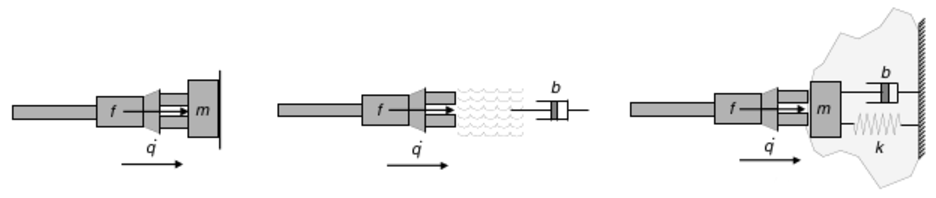
\includegraphics[scale=0.75]{type_of_impedances}
  \begin{itemize}
  \item[-] for each DoF the manipulator and the environment can be described using impedances $Z_m$ and $Z_e$
  \item[-] the environment is defined to be any element connected to or contacting the robot anywhere \textcolor{red}{\emph{past the wrist}} force sensor
  \item[-] $Z(\omega) = R(\omega) + j X(\omega)$
  \item[-] type of impedances
    \begin{itemize}
    \item[] inertial iff $|Z(0)| = 0$
    \item[] resistive iff $|Z(0)| = c \in (0, \infty)$
    \item[] capacitive iff $|Z(0)| = \infty$
    \end{itemize}
  \end{itemize}
\end{frame}

\begin{frame}
  \frametitle{Hybrid Impedance control}
  \framesubtitle{Duality principle for position control}
  Manipulator impedance chosen as the dual of the environment impedance
  \begin{columns}
    \begin{column}{0.5\columnwidth}
      \begin{flalign*}
        &v = \frac{Z_m(s)}{Z_m(s) + Z_e(s)}v_{des} - \frac{F_{env}}{Z_e + Z_m} &\\
      \end{flalign*}
    \end{column}
    \begin{column}{0.5\columnwidth}
      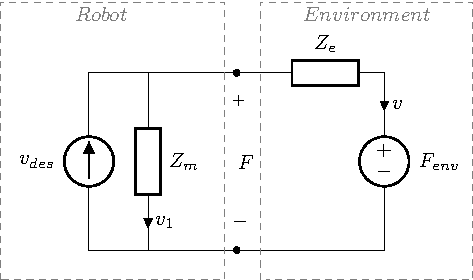
\includegraphics[width=\columnwidth]{position_control_model}
    \end{column}
  \end{columns}
  \begin{equation*}
    &e_{ss} \Big|_{F_{env}(t) \equiv 0} = \lim_{s \to 0}(v - v_{des}) = \frac{-Z_e(0)}{Z_m(0) + Z_e(0)} = 0 \text{ as long as } Z_m(0) \neq 0&
  \end{equation*}
  \begin{block}{Rule of thumb}
    inertial environments are position controlled with a noninertial manipulator impedances
  \end{block}
\end{frame}

\begin{frame}[shrink=10]
  \frametitle{Hybrid Impedance control}
  \framesubtitle{Position-Controlled subsystem}
  \begin{columns}
    \begin{column}{0.4\textwidth}
      \begin{align*}
        &v_{des} = v + v_1\\
        &v_1 = \frac{F}{Z_m}\\ 
        &F = Z_e v + F_{env}\\
        &a = \dot{v} = \frac{\mathrm{d}}{\mathrm{d}t} \left(v_{des} - \frac{F}{Z_m} \right)\\
        &Z_m = M s + \tilde{Z}_m\\
      \end{align*}
    \end{column}
    \begin{column}{0.5\textwidth}
      \centering
      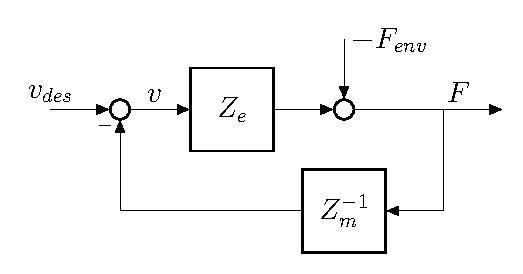
\includegraphics[scale=0.8]{position_control_feedback}
    \end{column}
  \end{columns}

  \begin{align*}
    &a = \frac{\mathrm{d}}{\mathrm{d}t} \left(v_{des} - \frac{F}{Ms + \tilde{Z}_m} \right) = \dot{v}_{des} - \frac{Fs}{Ms + \tilde{Z}_{m}} = \dot{v}_{des} - s v_1 \\
    &F = v_1 (Ms + \tilde{Z}_m) \quad v_1 = \frac{F - (v_{des} - v)\tilde{Z}_m}{Ms}\\
    &a = \dot{v}_{des} - s v_1 = \dot{v}_{des} - \cancel{s} \left( \frac{F - (v_{des} - v)\tilde{Z}_m}{M\cancel{s}} \right) = \dot{v}_{des} + \frac{(v_{des} - v)\tilde{Z}_m}{M} - \frac{F}{M}
  \end{align*}
\end{frame}

\begin{frame}
  \frametitle{Hybrid Impedance control}
  \framesubtitle{Duality principle for force control}
  Manipulator impedance chosen as the dual of the environment impedance
  \begin{columns}
    \begin{column}{0.5\columnwidth}
      \begin{flalign*}
        F = \frac{Z_e(s)}{Z_m(s) + Z_e(s)}F_{des} + \frac{Z_e Z_m}{Z_m + Z_e} V_{env}
      \end{flalign*}
    \end{column}
    \begin{column}{0.45\columnwidth}
      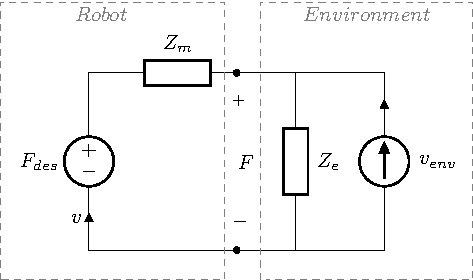
\includegraphics[width=\columnwidth]{force_control_model}
    \end{column}
  \end{columns}
  \begin{equation*}
    e_{ss} \Big|_{v_{env}(t) \equiv 0} = \lim_{s \to 0}(F - F_{des}) = \frac{-Z_m(0)}{Z_m(0) + Z_e(0)} = 0 \text{ as long as } Z_m(0) < \infty
  \end{equation*}
  \begin{block}{Rule of thumb}
    capacitive environments are force controlled with noncapacitive manipulator impedances
  \end{block}
\end{frame}

\begin{frame}[shrink=10]
  \frametitle{Hybrid Impedance control}
  \framesubtitle{Force-Controlled subsystem}
  \begin{columns}
    \begin{column}{0.4\textwidth}
      \begin{align*}
        &F = F_{des} + Z_m v\\
        &v = \frac{F - F_{des}}{Z_m}\\
        &F = Z_e(v + v_{env})\\
        &a = \dot{v} = \frac{\mathrm{d}}{\mathrm{d}t} \left(\frac{F - F_{des}}{Z_m} \right)\\
        &Z_m = M s + \tilde{Z}_m\\
      \end{align*}
    \end{column}
    \begin{column}{0.5\textwidth}
      \centering
      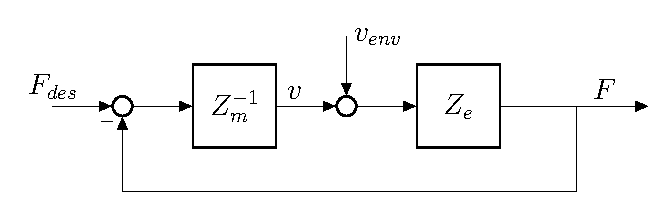
\includegraphics[scale=0.8]{force_control_feedback}
    \end{column}
  \end{columns}

  \begin{align*}
    &a = \frac{\mathrm{d}}{\mathrm{d}t} \left(\frac{F - F_{des}}{Ms + \tilde{Z}_m} \right) = \left(\frac{s(F - F_{des})}{Ms + \tilde{Z}_m} \right)\\
    &vMs + v \tilde{Z}_m = F - F_{des}\\
    &v = \frac{1}{Ms} (F - F_{des} - v \tilde{Z}_m )\\
    &a = \dot{v} = \frac{\cancel{s}}{M\cancel{s}} (F - F_{des}) - \frac{\cancel{s}}{M\cancel{s}}( \tilde{Z}_m v) = \frac{1}{M} (F - F_{des}) - \frac{1}{M}( \tilde{Z}_m v) \\
  \end{align*}
\end{frame}

\begin{frame}
  \frametitle{Hybrid Impedance control}
  \framesubtitle{Control assigned to each DoF}
  Position (${}^{ws}r_x,{}^{ws}r_y$):
  \begin{itemize}
  \item[-] inertial environment (manipulator moving a payload along given axis)
  \item[-] $Z_{m,p} = M_p s + \tilde{Z}_{m,p} = M_p s + B_p + \frac{K_p}{s}$
  \item[-] $a_{p} = a_{des,p} + \frac{B_p}{M_p} (v_{des,p} - v_p) + \frac{K_p}{M_p} (x_{des,p} - x_p) - \frac{F_p}{M_p}$
  \end{itemize}
  Attitude ($\psi$, $\theta$, $\phi$):
  \begin{itemize}
  \item[-] inertial environment (manipulator rotating a payload about given axis )
  \item[-] $Z_{m,a} = M_a s + \tilde{Z}_{m,a} = M_a s + B_a + \frac{K_a}{s}$
  \item[-] $a_a = a_{des,a} + \frac{B_a}{M_a} (v_{des,a} - v_a) + \frac{K_a}{M_a} (x_{des,a} - x_a)$
  \end{itemize}
  Force (${}^{ws}f_z$):
  \begin{itemize}
  \item[-] capacitive environment
  \item[-] $Z_{m,f} = M_f s + \tilde{Z}_{m,f} = M_f s + B_f$
  \item[-] $a_{f} = M_f^{-1}((f_{des} - f) - B_f v_z)$
  \end{itemize}  
\end{frame}

\begin{frame}
  \frametitle{Hybrid Impedance control}
  \framesubtitle{Filtering action}
  In principle one could assign a position control law \textcolor{red}{\emph{and}} a force
  control law for \textcolor{red}{\emph{each}} DoF
  
  A selection matrix $S$ is used to separate the force-controlled and position-controlled \emph{reciprocal} subspaces
  \begin{columns}
    \begin{column}{0.6\textwidth}
      \begin{flalign*}
        &\vec{a}_p = 
        \begin{bmatrix}
          a_{p,x} & a_{p,y} & a_{p,z}
        \end{bmatrix}^T&\\
        &\vec{a}_a = 
        \begin{bmatrix}
          a_{a, \psi} & a_{a, \theta} & a_{a, \phi}
        \end{bmatrix}^T&\\
        &\vec{a}_f = 
        \begin{bmatrix}
          a_{f,x} & a_{f,y} & a_{f,z} & a_{f, \psi} & a_{f, \theta} & a_{f, \phi}
        \end{bmatrix}^T&\\
        &\vec{a} = S 
        \begin{bmatrix}
          \vec{a}_p \\
          \vec{a}_a
        \end{bmatrix} + (I - S) \vec{a}_f&
      \end{flalign*}
    \end{column}
    \begin{column}{0.35\columnwidth}
      $
      S =
        \begin {bmatrix}
          1 & 0 & 0 & 0 & 0 & 0\\
          0 & 1 & 0 & 0 & 0 & 0\\
          0 & 0 & 0 & 0 & 0 & 0\\
          0 & 0 & 0 & 1 & 0 & 0\\
          0 & 0 & 0 & 0 & 1 & 0\\
          0 & 0 & 0 & 0 & 0 & 1\\
        \end {bmatrix}
      $
    \end{column}
  \end{columns}
\end{frame}

\begin{frame}
  \frametitle{Hybrid Impedance control}
  The resulting control law is
  \begin{align*}
    & a_x = \ddot{r}_{x,des} + B_x (\dot{r}_{x,des} - \dot{r}_x) + K_x (r_{x,des} - r_x) - F_x \\
    & a_y = \ddot{r}_{y,des} + B_y (\dot{r}_{y,des} - \dot{r}_y) + K_y (r_{y,des} - r_y) - F_y \\
    & a_z = - B_f \dot{r}_z + K_f(F_{z,des} - F_z) \\
    & a_{\psi} = - B_{\psi} \dot{\psi} + K_{\psi} (\psi_{des} - \psi) \\
    & a_{\theta} = - B_{\theta} \dot{\theta} + K_{\theta} (\theta_{des} - \theta) \\
    & a_{\phi} = - B_{\phi} \dot{\phi} + K_{\phi} (\phi_{des} - \phi)
  \end{align*}
\end{frame}

\begin{frame}
  \frametitle{Kinestatic filtering}
  \framesubtitle{A different interpretation of the selection matrix}
  Position controlled and force controlled subspaces can be seen in terms of
  \emph{natural} and \emph{artificial} constraints:
  \begin{itemize}
  \item[-]natural: directions along which the end effector can not move and exert forces
  \item[-]artificial: directions along which the end effector can move and exert forces
  \end{itemize}

  Artificial constraints directions belong to the span of appropriate matrices
\end{frame}

\begin{frame}
  \frametitle{Kinestatic filtering}
  \framesubtitle{An example}
  Consider twists and wrenches projected in $ws$
  \begin{columns}
    \begin{column}{0.35\textwidth}
      $
      B=
      \begin {bmatrix}
        1 & 0 & 0 & 0 & 0\\
        0 & 1 & 0 & 0 & 0\\
        0 & 0 & 0 & 0 & 0\\
        0 & 0 & 1 & 0 & 0\\
        0 & 0 & 0 & 1 & 0\\
        0 & 0 & 0 & 0 & 1\\
      \end {bmatrix}
      $
    \end{column}
    \begin{column}{0.35\columnwidth}
      $
      a=
      \begin {bmatrix}
        0 \\
        0 \\
        1 \\
        0 \\
        0 \\
        0 \\
      \end {bmatrix}
      $
    \end{column}
  \end{columns}
  \centering
  \begin{equation*}
    {}^{ws}\boldsymbol{\xi}_{adm} \in \mathcal{R}(B)
    ,\quad
    {}^{ws}\vec{w}_{adm} \in \mathcal{R}(a)
  \end{equation*}
  \vskip-0.7em
  \begin{block}{}
    The most general motion is that of a translation ($x$-$y$ direction of $ws$)
    and/or a rotation about some axis that pass through a point $P$, tipically the tip of the
    end effector E.
  \end{block}
  \begin{block}{}
    Force can only be exerted along the $z$ direction of $ws$. No torques are allowed.
  \end{block}


\end{frame}

\begin{frame}
  \frametitle{Kinestatic filtering}
  \framesubtitle{An example}
  In order to filter out undesired twists and wrenches the following projection matrices are used
  \begin{columns}[t]
    \begin{column}{0.4\columnwidth}
      \begin{flalign*}
        &P_B = B (B^T B)^{-1} B^T\\
        &P_B \vec{e}_i = \vec{e}_i \quad i \in \{1, 2, 4, 5, 6\}\\
        &P_B \vec{e}_3 = \vec{0}\\
      \end{flalign*}
    \end{column}
    \begin{column}{0.4\columnwidth}
      \begin{flalign*}
        &P_a = a (a^T a)^{-1} a^T&\\
        &P_a \vec{e}_i = \vec{0} \quad i \in \{1, 2, 4, 5, 6\}\\
        &P_a \vec{e}_3 = \vec{e}_3\\
      \end{flalign*}
    \end{column}
  \end{columns}

  The projectors lead to the selection matrices $S = P_B$ and $I-S = P_a$
\end{frame}

\begin{frame}
  \frametitle{Kinestatic filtering}
  \framesubtitle{A more general example}
  In general twists/wrenches can be commanded with respect to a
  different reference point $E'$ for example $EE' = \begin{bmatrix} \bar{x} & 0 & 0 \end{bmatrix}^T$
  \begin{columns}
    \begin{column}{0.4\columnwidth}
      \begin{flalign*}
        &{}^{ws}\boldsymbol{\xi}' = K(\bar{x}) ({}^{ws}\boldsymbol{\xi})\\
        &B' = K B =
        \left[
          \begin{smallmatrix}
            1 & 0 & 0 & 0 & 0 \\
            0 & 1 & 0 & 0 & x \\
            0 & 0 & 0 & -x & 0 \\
            0 & 0 & 1 & 0 & 0 \\
            0 & 0 & 0 & 1 & 0 \\
            0 & 0 & 0 & 0 & 1 \\
          \end{smallmatrix}
          \right]\\
      \end{flalign*}
    \end{column}
    \begin{column}{0.4\columnwidth}
      \begin{flalign*}
        &{}^{ws}\vec{w}' = G(\bar{x}) ( {}^{ws}\vec{w})\\
        &a' = G a =
        \left[
          \begin{smallmatrix}
            0 \\
            0 \\
            1 \\
            0 \\
            x \\
            0 \\
          \end{smallmatrix}
          \right]\\
      \end{flalign*}
    \end{column}
  \end{columns}
  However using the standard projector gives for example
  \begin{columns}
    \begin{column}{0.4\columnwidth}
      \begin{flalign*}
        &P_B' K \vec{e}_3 =
        \left[
          \begin{smallmatrix}
            0 & 0 & \textcolor{red}{\frac{x^2}{x^2+1}} & 0 & \textcolor{red}{-\frac{x}{x^2+1}} & 0\\
          \end{smallmatrix}
          \right]^T
      \end{flalign*}
    \end{column}
    \begin{column}{0.4\columnwidth}
      \begin{flalign*}
        &P_a' G \vec{e}_5 =
        \left[
          \begin{smallmatrix}
            0 & 0 & \textcolor{red}{\frac{x}{x^2+1}} & 0 & \textcolor{red}{\frac{x^2}{x^2+1}} & 0\\
          \end{smallmatrix}
          \right]^T
      \end{flalign*}
    \end{column}
  \end{columns}
\end{frame}

\begin{frame}
  \frametitle{Kinestatic filtering}
  \framesubtitle{An invariant filter [Marescotti, Bonivento and Melchiorri, 1990]}
  \begin{columns}
    \begin{column}{0.4\columnwidth}
      \begin{flalign*}
        &P_B'' = K P_B K^{-1}
      \end{flalign*}
      \begin{flalign*}
        \text{If } & P_B ({}^{ws}\boldsymbol{\xi}) = {}^{ws}\boldsymbol{\xi}\\
        \text{then } &P_B' ({}^{ws}\boldsymbol{\xi}') = P_B' K ({}^{ws}\boldsymbol{\xi}) \\
        &=K P_B K^{-1} K ({}^{ws}\boldsymbol{\xi})\\
        &=K P_B ({}^{ws}\boldsymbol{\xi})\\
        &=K ({}^{ws}\boldsymbol{\xi}) = {}^{ws}\boldsymbol{\xi}'
      \end{flalign*}
      \begin{flalign*}
        \text{If } & P_B ({}^{ws}\boldsymbol{\xi}) = \vec{0}\\
        \text{then } &P_B' ({}^{ws}\boldsymbol{\xi}') =K P_B ({}^{ws}\boldsymbol{\xi})\\
        &= \vec{0}
      \end{flalign*}
    \end{column}
    \begin{column}{0.4\columnwidth}
      \begin{flalign*}
        &P_a'' = G P_a G^{-1}
      \end{flalign*}
      \begin{flalign*}
        \text{If } & P_a ({}^{ws}\vec{w}) = {}^{ws}\vec{w}\\
        \text{then } &P_a' ({}^{ws}\vec{w}') = P_a' G ({}^{ws}\vec{w}) \\
        &=G P_a G^{-1} G ({}^{ws}\vec{w})\\
        &=G P_a ({}^{ws}\vec{w})\\
        &=G ({}^{ws}\vec{w}) = {}^{ws}\vec{w}'
      \end{flalign*}
      \begin{flalign*}
        \text{If } & P_a ({}^{ws}\vec{w}) = \vec{0}\\
        \text{then } &P_a' ({}^{ws}\vec{w}') =G P_a ({}^{ws}\vec{w})\\
        &= \vec{0}
      \end{flalign*}
    \end{column}
  \end{columns}
\end{frame}

\begin{frame}[shrink=10]
  \frametitle{Kinestatic filtering}
  \framesubtitle{Combining HIC with the kinestatic filtering}
  Since the kinestatic filtering is applied to twists and wrenches
  it is not possible to apply it directly to the commanded accelerations
  described above.\\
  Anyway, as observed in [Marescotti, Bonivento and Melchiorri, 1990],
  there is no necessity to use the alternative projectors $P_B''$ and
  $P_a''$ in the control algorithm since twists and wrenches expressed
  with respect to another reference point can always be transformed back
  to their original form using the inverse transformations $K^{-1}$ and
  $G^{-1}$.\\
  In that case the projection matrices always reduce to the selection matrices
  $S$ and $I-S$ that are also suitable to filter undesired commanded accelerations.
  \center{
    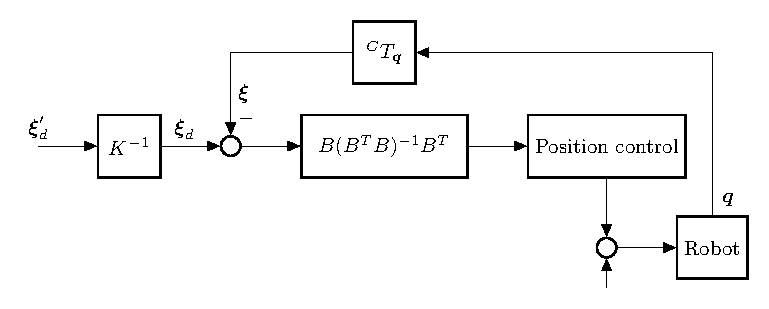
\includegraphics[scale=0.8]{kinestatic_filtering}
    }
\end{frame}

\begin{frame}{Issues with internal motions}
  In the case of the task described the Kuka LWR $4+$ is a kinetically redundant manipulator.
  \par
  Extensive simulations revealed
  that the uncontrolled internal motions of the robot, while not affecting the
  desired attitude of the hand, cause the $5$-th and $7$-th links to rotate
  cooperatively and reach their limits soon. Another issue with internal motions
  is that they could cause, in some situations, collisions between the $4$-th
  link and the table which is part of the workspace of the robot.
  \par
  These issues are solved use a \emph{dynamically consistent} generalized inverse of the Jacobian [Khatib, 1987]
\end{frame}
  
\begin{frame}{Control of internal motions [Khatib, 1987]}
  The standard operational space dynamics can be written by substituting
  (\ref{eq:dynamic_joint}) in (\ref{eq:xddot}) resulting in (\ref{eq:operational_space_dyn})
  \begin{columns}
    \begin{column}{0.7\columnwidth}
      \begin{equation}\label{eq:dynamic_joint}
      B(\vec{q}) \ddot{\vec{q}} + C(\vec{q}, \dot{\vec{q}}) \dot{\vec{q}} + \vec{G}(\vec{q}) = \vec{\tau} = J^{T} \vec{\gamma}
      \end{equation}
      \begin{equation}\label{eq:xddot}
        \vec{\ddot{x}} = J(\vec{q}) \vec{\ddot{q}} + \vec{h}(\vec{q},\vec{\dot{q}})
      \end{equation}
      \begin{equation}\label{eq:operational_space_dyn}
        \Lambda \vec{\ddot{x}} + \vec{\mu}(\vec{q}, \vec{\dot{q}}) + \vec{p} = \vec{\gamma}
      \end{equation}
    \end{column}
    \begin{column}{0.4\columnwidth}
      \[
      \begin{split}
        &\Lambda = (J B^{-1} J^{T})^{-1}\\
        &\vec{\mu} = \bar{J}^{T} C \vec{\dot{q}} - \Lambda \vec{h}\\
        &\vec{p} = \bar{J}^T \vec{G}\\
        &\bar{J} = B^{-1} J^{T} \Lambda
      \end{split}
      \]
    \end{column}
  \end{columns}
  %% The matrix 
  %% which solves the problem of finding the joints velocities that produce a desired twist
  %% while minimizing the manipulator's instantaneous kinetic energy.
The equation (\ref{eq:operational_space_dyn}) can also be written in the form
\[
\bar{J}^{T} (B \vec{\ddot{q}} + C \vec{\dot{q}} + \vec{G}) = \vec{\gamma}
\]
resulting in 
\[
\vec{\gamma} = \bar{J}^{T} \vec{\tau}
\]
i.e. $\bar{J} = B^{-1} J^{T} \Lambda$ is a dynamically consistent generalized inverse of the Jacobian matrix
\end{frame}

\begin{frame}{Control of internal motions [Khatib, 1987]}
 In order to control the undesired internal motions a command torque $\vec{\tau}$ of the form
 \[
 \vec{\tau} = J^{T} \vec{\gamma} + (I_7 - J^{T}\bar{J}^{T}) \vec{\gamma}_{0}
 \]
 can be used where $\vec{\gamma}_{0}$ is projected in the null space of $\bar{J}^{T}$ hence not affecting
 the command wrench seen by the hand
 \par
 The final control law is
 \[
 \vec{\tau} = C \dot{\vec{q}} + \vec{G} + {}^{b}J^{T}_{S} ( B_A \vec{a} - B_A {}^{ws} \dot{J_{A,E}} \dot{\vec{q}} + {}^b\vec{w}_{S}) +
 (I_7 - ({}^{b}J^{T}_{S}) ({}^{b} \bar{J}^{T}_{S})) \vec{\gamma}_{0}
 \]
where
\[
\prescript{b}{}{\bar{J}}_{S} = B^{-1} ({}^{b} J^{T}_{S}) ({}^{b} \Lambda_{S}) \quad 
\prescript{b}{}{\Lambda}_{S} = ({}^{b} J_{S} B^{-1} ({}^{b} J^{T}_{S}))^{-1}
\]
\end{frame}

\begin{frame}{Design of the null operational wrench command $\vec{\gamma}_{0}$}
  To fix the orientation of the $5$-th link and
  to regulate the altitude between the $4$-th link and the hand 
  $\vec{\gamma}_0$ is chosen
  \[
  \vec{\gamma}_{0} = J_{im} ^{T} (K_p (\vec{x}_{im,des} - \vec{x}_{im} ) - K_d \vec{\dot{x}}_{im})
  \]
  \[
  \vec{x}_{im} =
  \begin{bmatrix}
    {}^{b} x_{l4} & {}^{b} y_{l4} & {}^{b} z_{l4} & \psi_{l5} & \theta_{l5} & \phi_{l5}
  \end{bmatrix}^{T} =
  \begin{bmatrix}
    \vec{p}^{T}_{l4} & \vec{\Phi}^{T}_{l5}
  \end{bmatrix}^{T}
  \]
  \[
  \begin{bmatrix}
  \vec{\dot{p}}_{l4} \\
  \vec{\dot{\Phi}}_{l5} \\
  \end{bmatrix} =
  J_{im} \vec{\dot{q}}
  \]
  \par
  \[
  K_p = \text{diag}(0, 0, k_{p,z}^{im}, 0, 0, k_{p, att}^{im})
  \quad
  K_d = k_{d}^{im} I_{6}
  \]
  \[
  \vec{p}_{l4} =
  \begin{bmatrix}
    * & * & {}^{b} p_{ee_{z}} + off_z
  \end{bmatrix}^{T}
  \quad
  \vec{\Phi}_{l5} =
  \begin{bmatrix}
    * & * & 0
  \end{bmatrix}^{T}
  \]
\end{frame}

\section{Approaching phase controller}
As explained in the section \ref{sec:task_division} before the execution of the dragging phase
a preliminar approaching phase is required  to move the hand near the object of interest.
\par
In principle the HIC controller could also be used to perform this task but in practice
some issues due to the singularity introduced by the Euler ZYZ parametrization and due to the
joints limits make that controller useful during the dragging phase only where short movements are executed
and the attitude is carefully commanded to avoid the singularity issue.
So another controller was developed using a joint space approach so that large movements can be performed.

\subsection{Design of a joint space point to point controller}
The alternative controller was developed combining an inverse dynamics controller in joint
space with an inverse kinematics solver.
\par
By substituing a command torque of the form
\[
\vec{\tau} = C(\vec{q}, \dot{\vec{q}}) \dot{\vec{q}} + \vec{G}(\vec{q}) + B(\vec{q}) \vec{a}
\]
in the joint space dynamics of the manipulator
\[
  B(\vec{q})\ddot{\vec{q}} + C(\vec{q}, \dot{\vec{q}}) \dot{\vec{q}} + \vec{G}(\vec{q}) = \vec{\tau}
\]
the following results
\[
\ddot{\vec{q}} = \vec{a}_{p2p}
\]
where $\vec{a}_{p2p}$ is the new input vector.
\par
In order to move the hand from the previous configuration $\vec{q}_{prev}$
to a new one expressed as a position in cartesian coordinates $\vec{p}_{ee}$ and
an orientation $\prescript{b}{}{R}_{ee}$ a joint space trajectory was generated
\[
q_{des}^{i}(t) = a_0 + a_1 t + a_2 t^2 + a_3 t^3 + a_4 t^4 + a_5 t^5
\]
with boundary conditions
\[
\begin{split}
  &q_{des}^{i}(0) = q_{prev}^{i} \quad \dot{q}_{des}^{i}(0) = 0 \quad \ddot{q}_{des}^{i}(0) = 0\\
  &q_{des}^{i}(t_f) = q_{f}^{i} \quad \dot{q}_{des}^{i}(t_f) = 0 \quad \ddot{q}_{des}^{i}(t_f) = 0
\end{split}
\]
where $\vec{q}_{f}$ is given by an inverse kinematics solver
\[
\vec{q}_{f} = FK^{-1}(\vec{p}_{ee,des},\prescript{b}{}{R}_{ee,des})
\]
and is discarded whenever its components exceed the joints limits.
\par
In order to execute the trajectory an input vector of the form
\[
\vec{a}_{p2p} = \ddot{\vec{q}}_{des} + K_d(\dot{\vec{q}}_{des} - \dot{\vec{q}}) + K_p(\vec{q}_{des} - \vec{q})
\]
was used where $K_p$ and $K_d$ are positive definite matrices.
\newpage

\begin{frame}
  \frametitle{Simulation setup}
  \begin{itemize}
  \item[-] emulated Kuka FRI Joint specific impedance control mode
    \begin{itemize}
    \item[] $\boldsymbol{\tau}_{cmd} = K_j(\vec{q}_{FRI} - \vec{q}_{msr}) + D(d_{j}) + \boldsymbol{\tau}_{FRI} + \vec{f}_{dynamics}(\vec{q}, \dot{\vec{q}}, \ddot{\vec{q}})$
    \end{itemize}
  \item[-] $K_j = 0$
  \item[-] $\vec{q}_{FRI} = \vec{q}_{msr}$
  \item[-] $d_{j} = 0$
  \item[-] $\vec{f}_{dynamics}(\vec{q}, \dot{\vec{q}}, \ddot{\vec{q}})$ supposed to be $\vec{G}(\vec{q})$ evaluated using KDL library
  \item[-] $\boldsymbol{\tau}_{FRI}$ used as commanded torque
  \item[-] controller @ $1$kHz
  \end{itemize}

\end{frame}

\begin{frame}
  \frametitle{Simulation setup}
  \framesubtitle{Issues}
  \begin{flalign*}
    &\boldsymbol{\tau}_{FRI} = C \dot{\vec{q}} +  B\vec{a}_{app}(\vec{\dot{q}})\\
    &\boldsymbol{\tau}_{FRI} = C \dot{\vec{q}} + J^{T}_{F} ( B_A \vec{a}_{hic}(\vec{w}_{F}, \dot{\vec{q}}) - B_A \dot{J_{A,E}} \vec{\dot{q}} + \vec{w}_{F}) + \boldsymbol{\tau}_{null}(J_{a_{4}})
  \end{flalign*}
  
  \begin{itemize}
  \item[-] $B$ given by KDL {\color{dgreen}\cmark}
  \item[-] $C \dot{\vec{q}}$ given by KDL {\color{dgreen}\cmark}
    
  \item[-] only $\vec{q}$ is available (as in the real scenario)
    \begin{itemize}
    \item[-] $\dot{\vec{q}}$ estimated using an exponential smoothing {\color{orange}\cmark}
    \end{itemize}
    
  \item[-] Jacobians are evalutated using KDL library {\color{dgreen}\cmark} 

    \item[-] $\vec{w}_F$ given by force/torque sensor plugin (software)
      \begin{itemize}
      \item[-] corrupted signal when the tool is mounted on the wrist $\longrightarrow$ massless tool{\color{orange}\cmark}
    \end{itemize}
    \item[-] joints friction and contact friction neglected for ease of simulation {\color{orange}\cmark}
  \end{itemize}
\end{frame}

\begin{frame}
  \frametitle{Simulation setup}
  \framesubtitle{Approaching phase}
  \begin{itemize}
  \item[-] initial configuration: $\begin{bmatrix} -0.71 & 1.15 & 0.39 & 0.52 & -0.54 & -1.57 \end{bmatrix}$
  \item[-] final configuration: $\begin{bmatrix} 0.00 & -0.14 & 0.10 & 0.00 & 3.14 & 0.00 \end{bmatrix}$
  \item[-] duration $5$s
  \item[-] $K_p = \mathrm{diag}(30)$
  \item[-] $K_d = \mathrm{diag}(30)$
  \end{itemize}
\end{frame}

\begin{frame}
  \frametitle{Simulation setup}
  \framesubtitle{Approaching phase - Results}
  \begin{center}
   \vskip-0.1in
    \begin{tabular}{cc}
      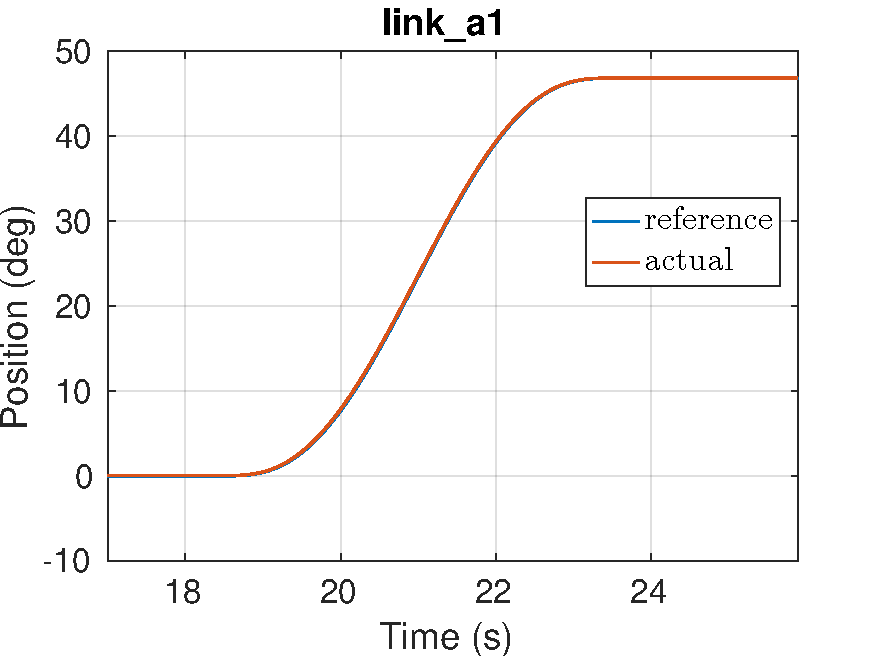
\includegraphics[scale=0.34]{cart_sim_a1} &
      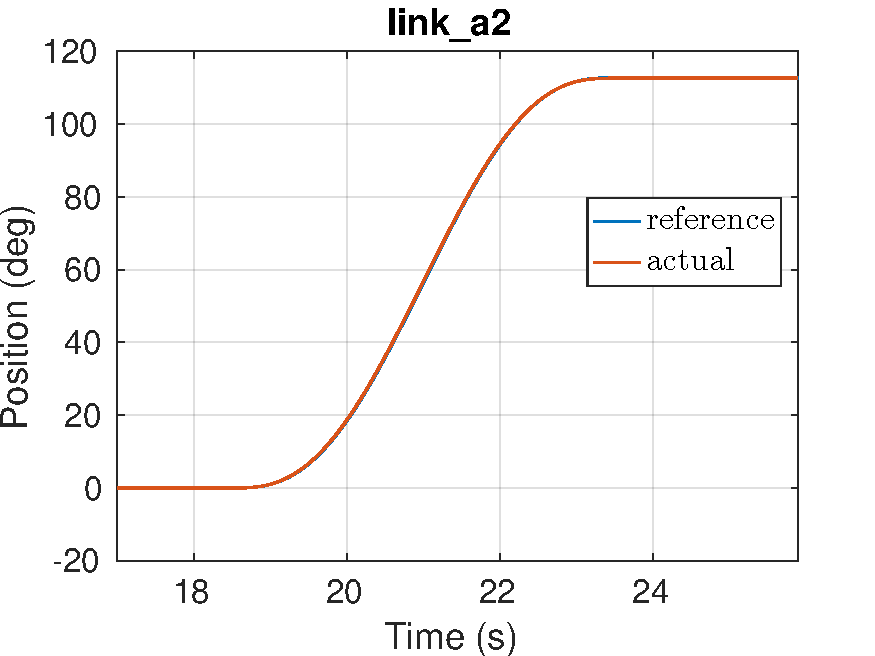
\includegraphics[scale=0.34]{cart_sim_a2}
    \end{tabular}
  \end{center}
  \begin{center}
   \vskip-0.1in
    \begin{tabular}{cc}
      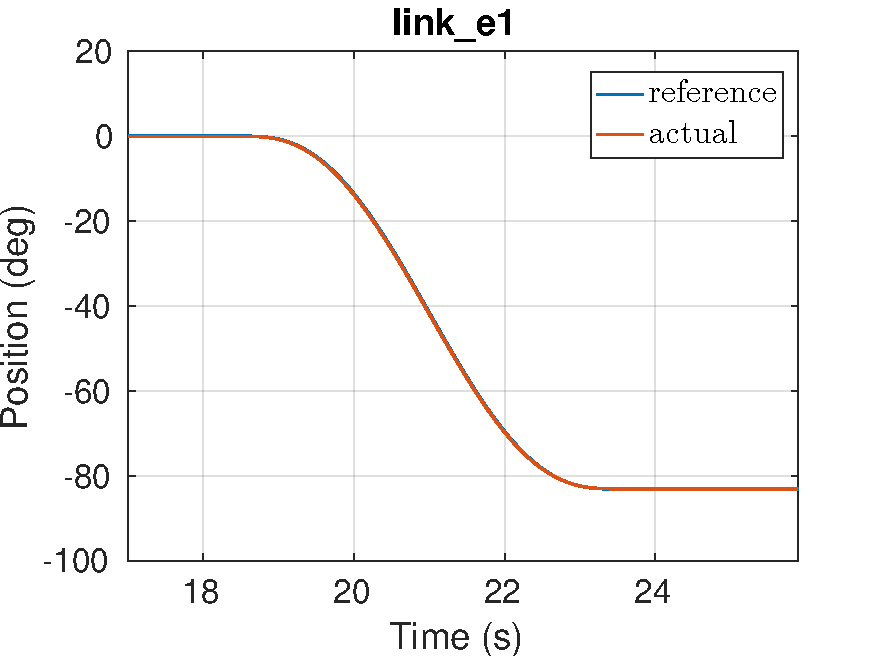
\includegraphics[scale=0.34]{cart_sim_e1} &
      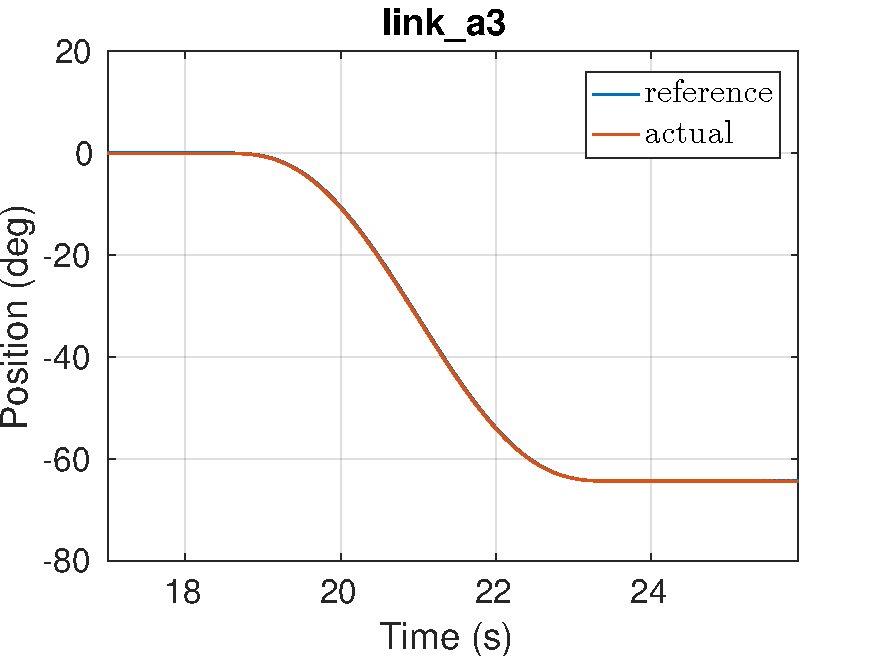
\includegraphics[scale=0.34]{cart_sim_a3}
    \end{tabular}
  \end{center}
\end{frame}

\begin{frame}
  \frametitle{Simulation setup}
  \framesubtitle{Approaching phase - Results}
  \begin{center}
   \vskip-0.1in
    \begin{tabular}{cc}
      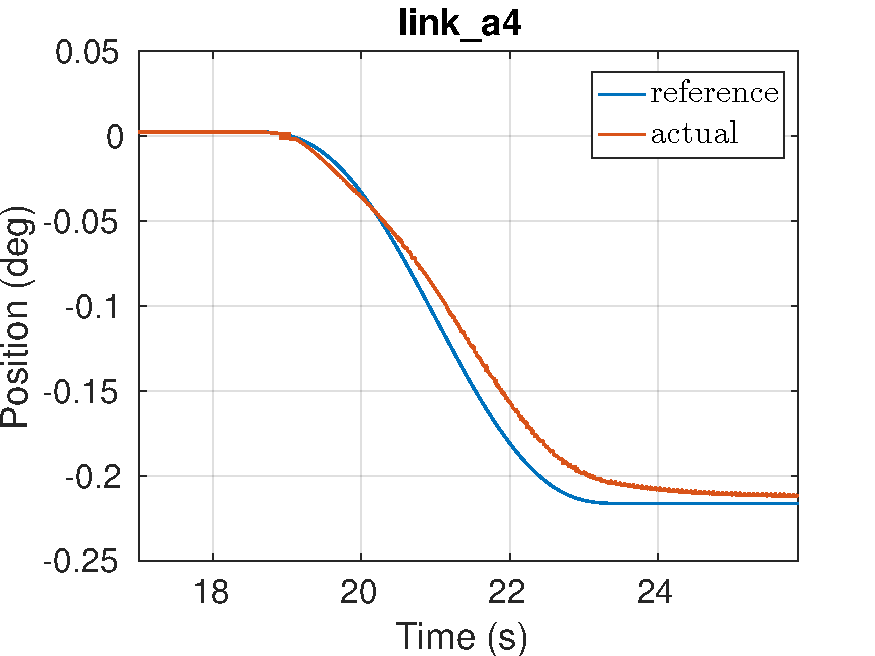
\includegraphics[scale=0.34]{cart_sim_a4} &
      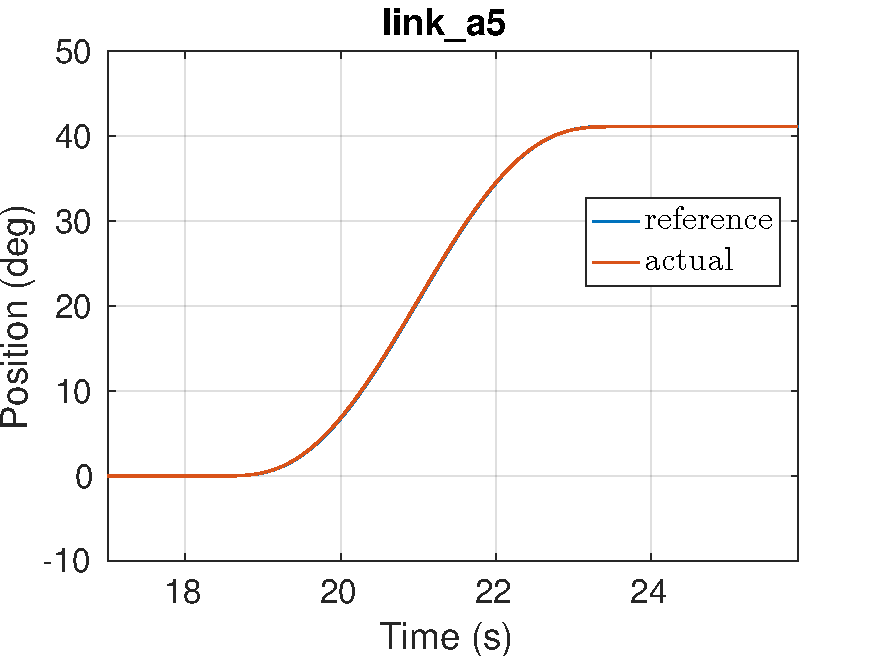
\includegraphics[scale=0.34]{cart_sim_a5}
    \end{tabular}
  \end{center}
  \begin{center}
   \vskip-0.1in
    \begin{tabular}{c}
      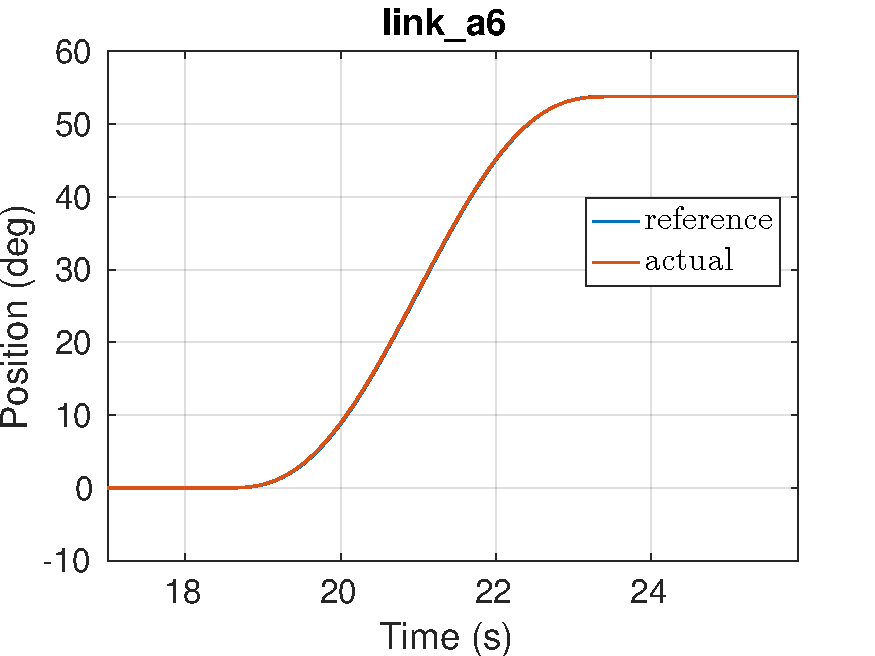
\includegraphics[scale=0.34]{cart_sim_a6}
    \end{tabular}
  \end{center}
\end{frame}

\begin{frame}
  \frametitle{Simulation setup}
  \framesubtitle{Force regulation}
  \begin{itemize}
  \item[-] duration $2$s
  \item[-] $K_p = \mathrm{diag}(30)$
  \item[-] $K_d = \mathrm{diag}(30)$
  \item[-] $k_{f} = 2$
  \item[-] $b_f = 25$
  \end{itemize}
\end{frame}

\begin{frame}
  \frametitle{Simulation setup}
  \framesubtitle{Force regulation- Results}
  \begin{center}
   \vskip-0.1in
    \begin{tabular}{cc}
      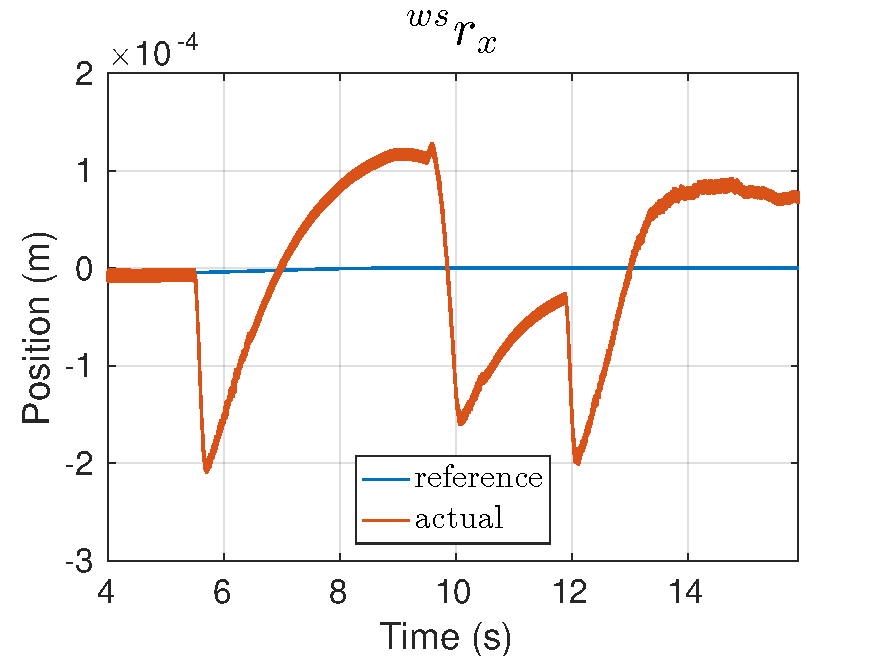
\includegraphics[scale=0.34]{force_sim_1_x} &
      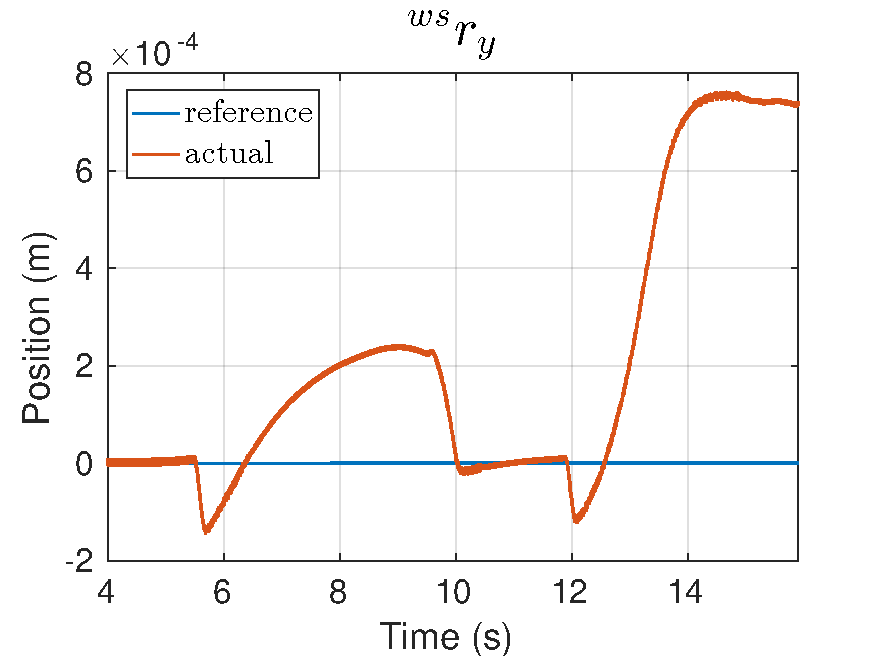
\includegraphics[scale=0.34]{force_sim_1_y}
    \end{tabular}
  \end{center}
  \begin{center}
   \vskip-0.1in
    \begin{tabular}{c}
      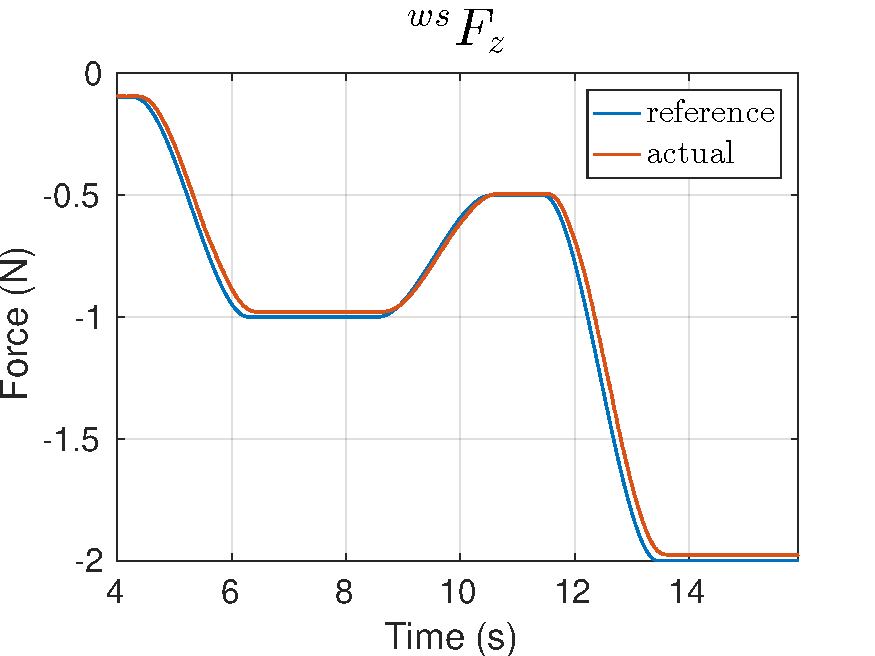
\includegraphics[scale=0.34]{force_sim_1_z}
    \end{tabular}
  \end{center}
\end{frame}

\begin{frame}
  \frametitle{Simulation setup}
  \framesubtitle{Force regulation + motion}
  \begin{itemize}
  \item[-] reference trajectory duration $5$s
  \item[-] reference force duration $2$s
  \item[-] $K_p = \mathrm{diag}(30)$
  \item[-] $K_d = \mathrm{diag}(30)$
  \item[-] $k_{f} = 2$
  \item[-] $b_f = 25$
  \end{itemize}
\end{frame}

\begin{frame}
  \frametitle{Simulation setup}
  \framesubtitle{Force regulation + motion - Results}
  \begin{center}
   \vskip-0.1in
    \begin{tabular}{cc}
      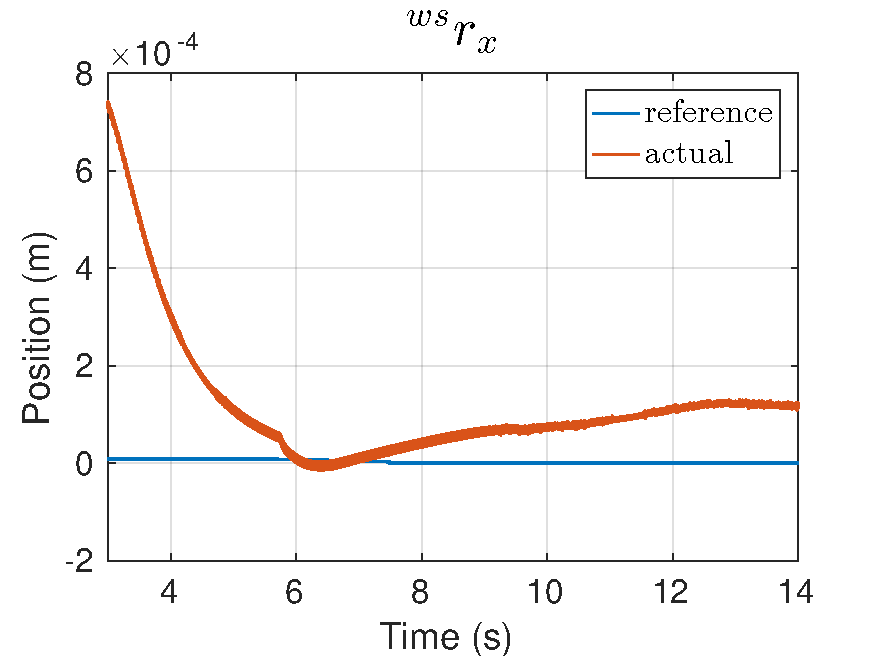
\includegraphics[scale=0.34]{force_sim_2_x} &
      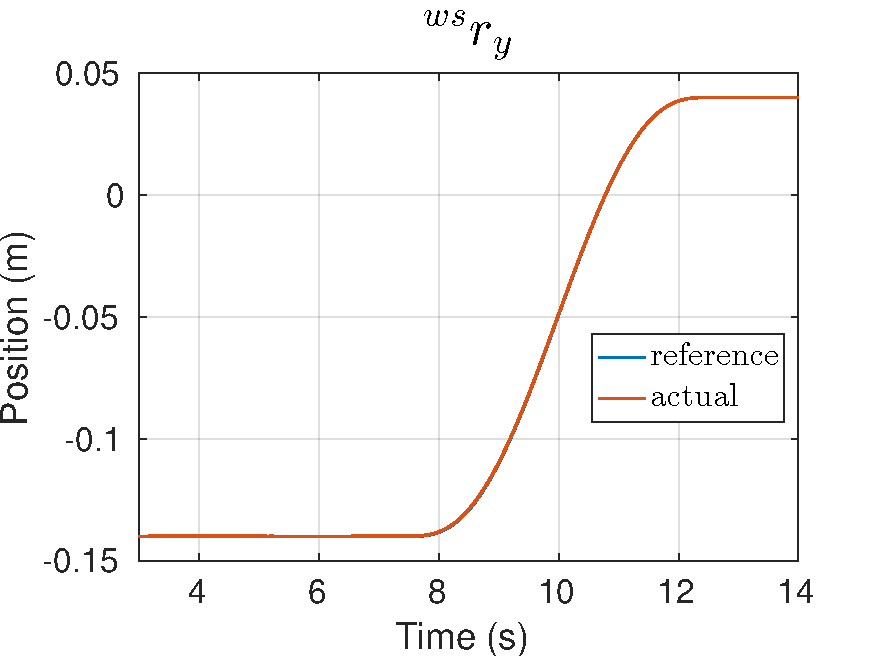
\includegraphics[scale=0.34]{force_sim_2_y}
    \end{tabular}
  \end{center}
  \begin{center}
   \vskip-0.1in
    \begin{tabular}{c}
      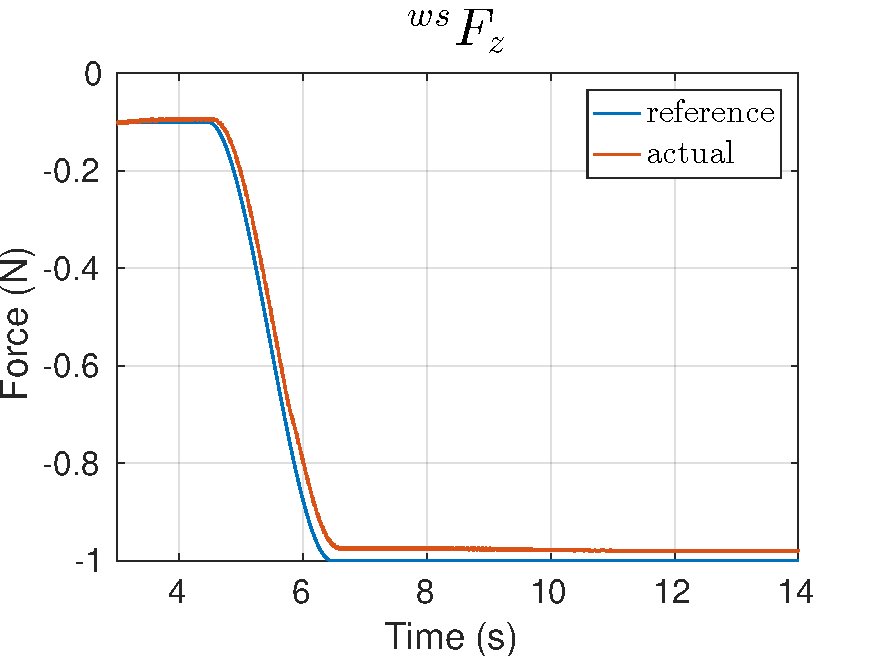
\includegraphics[scale=0.34]{force_sim_2_z}
    \end{tabular}
  \end{center}
\end{frame}

\begin{frame}
  \frametitle{Experimental setup}
  \begin{itemize}
  \item[-] Kuka FRI Joint specific impedance control mode
    \begin{itemize}
    \item[] $\boldsymbol{\tau}_{cmd} = K_j(\vec{q}_{FRI} - \vec{q}_{msr}) + D(d_{j}) + \boldsymbol{\tau}_{FRI} + \vec{f}_{dynamics}(\vec{q}, \dot{\vec{q}}, \ddot{\vec{q}})$
    \end{itemize}
  \item[-] $K_j = 0$
  \item[-] $\vec{q}_{FRI} = \vec{q}_{msr}$
  \item[-] $d_{j} = 0$
  \item[-] $\vec{f}_{dynamics}(\vec{q}, \dot{\vec{q}}, \ddot{\vec{q}})$ supposed to be $\vec{G}(\vec{q})$
  \item[-] $\boldsymbol{\tau}_{FRI}$ used as commanded torque
  \end{itemize}
\end{frame}

\begin{frame}
  \frametitle{Experimental setup}
  \framesubtitle{Issues}
  \begin{flalign*}
    &\boldsymbol{\tau}_{FRI} = C \dot{\vec{q}} +  B\vec{a}_{app}(\vec{\dot{q}})\\
    &\boldsymbol{\tau}_{FRI} = C \dot{\vec{q}} + J^{T}_{F} ( B_A \vec{a}_{hic}(\vec{w}_{F}, \dot{\vec{q}}) - B_A \dot{J_{A,E}} \vec{\dot{q}} + \vec{w}_{F}) + \boldsymbol{\tau}_{null}(J_{a_{4}})
  \end{flalign*}
  
  \begin{itemize}
    \item[-] masses, inertias and CoM of links are not extact:
      \begin{itemize}
      \item[-] $B$ given by FRI {\color{dgreen}\cmark}
      \item[-] $C \dot{\vec{q}}$ neglected {\color{red}\xmark}
      \end{itemize}
      
      \item[-] only $\vec{q}$ is available
      \begin{itemize}
      \item[-] $\dot{\vec{q}}$ estimated using an exponential smoothing {\color{orange}\cmark}
      \end{itemize}
        
    \item[-] Jacobians are evalutated using KDL library {\color{dgreen}\cmark} 

    \item[-] $\vec{w}_F$ given by force/torque sensor
      \begin{itemize}
      \item[-] $\vec{w}_F = \vec{w}_{ideal} + \vec{w}_{offs}$ (offset not yet estimated) {\color{red}\xmark}
      \item[-] problems with light sensitivity! {\color{dgreen}\cmark}
    \end{itemize}
    \item[-] friction {\color{red}\xmark}
  \end{itemize}
\end{frame}

\begin{frame}
  \frametitle{Experimental setup}
  \framesubtitle{Approaching phase}
  \begin{itemize}
  \item[-] initial configuration: 
  \item[-] final configuration: 
  \item[-] duration $5$s
  \item[-] $K_p = \mathrm{diag}(1600)$
  \item[-] $K_d = \mathrm{diag}(30)$
  \end{itemize}
\end{frame}

\begin{frame}
  \frametitle{Experimental setup}
  \framesubtitle{Approaching phase - Results}
  \begin{center}
   \vskip-0.1in
    \begin{tabular}{cc}
      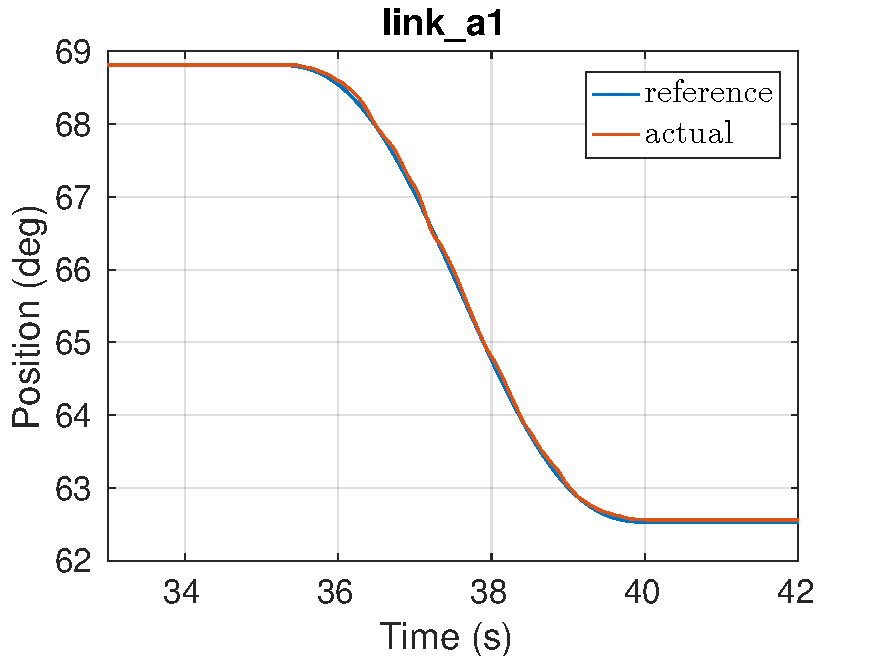
\includegraphics[scale=0.34]{cart_real_3_a1} &
      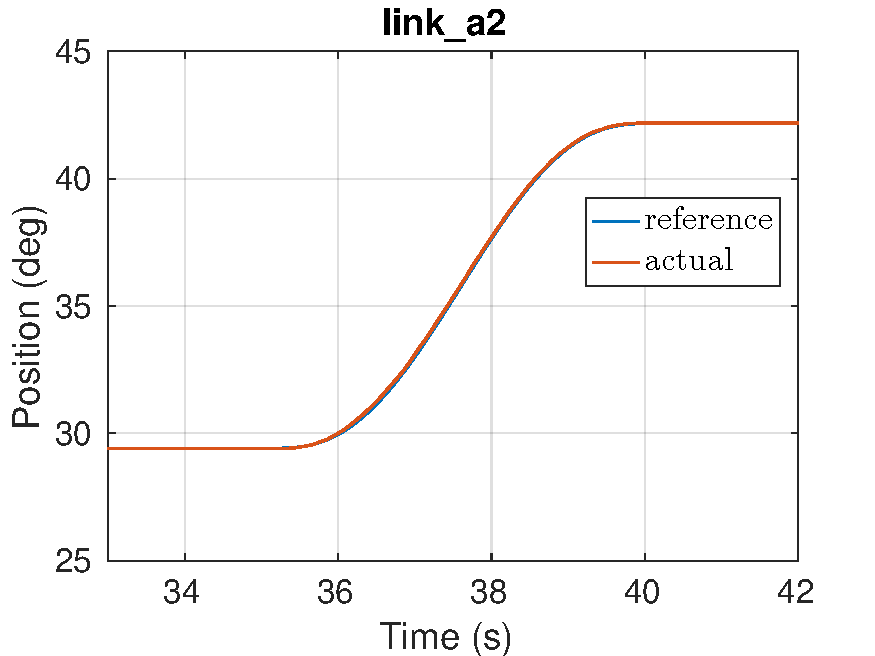
\includegraphics[scale=0.34]{cart_real_3_a2}
    \end{tabular}
  \end{center}
  \begin{center}
   \vskip-0.1in
    \begin{tabular}{cc}
      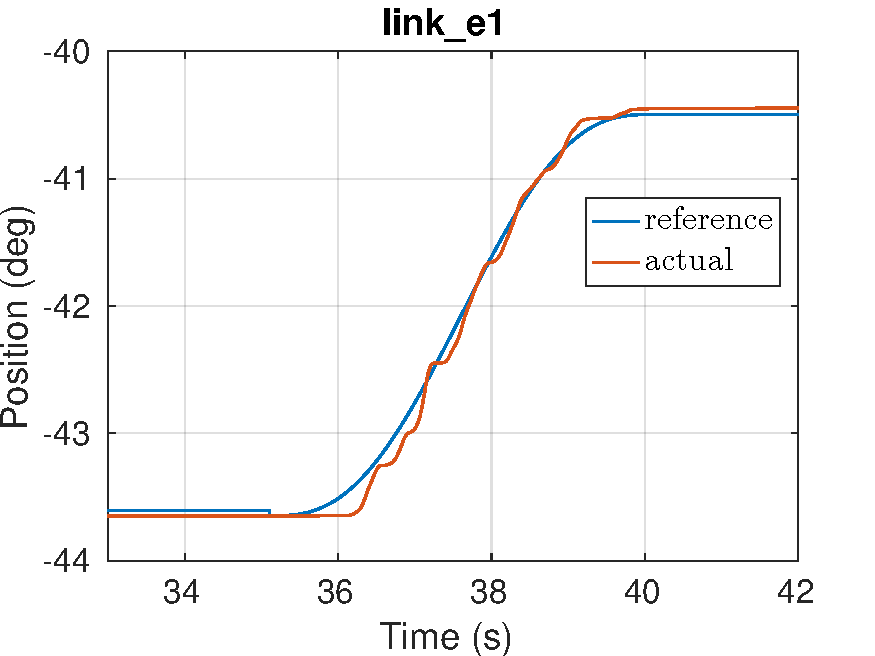
\includegraphics[scale=0.34]{cart_real_3_e1} &
      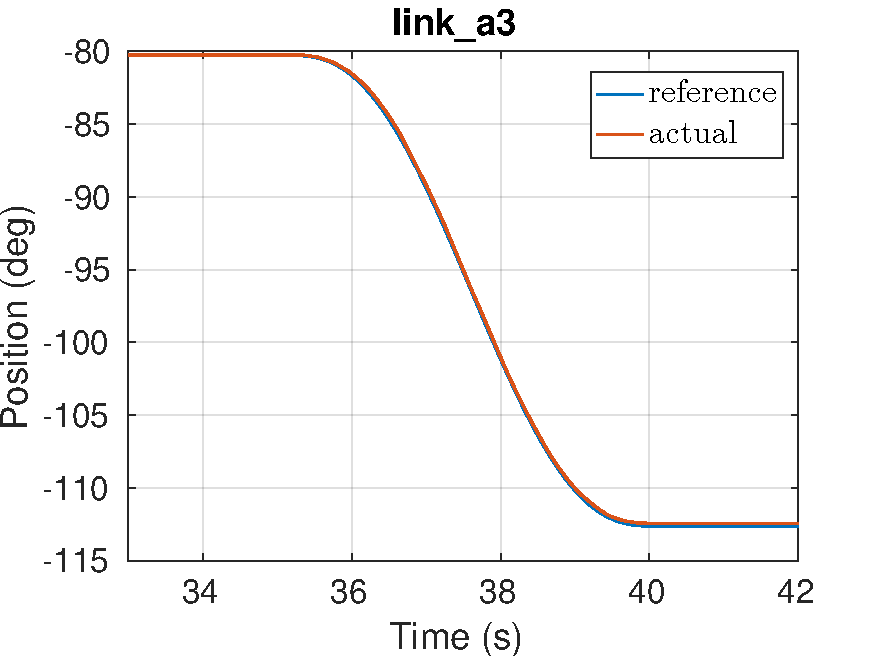
\includegraphics[scale=0.34]{cart_real_3_a3}
    \end{tabular}
  \end{center}
\end{frame}

\begin{frame}
  \frametitle{Experimental setup}
  \framesubtitle{Approaching phase - Results}
  \begin{center}
   \vskip-0.1in
    \begin{tabular}{cc}
      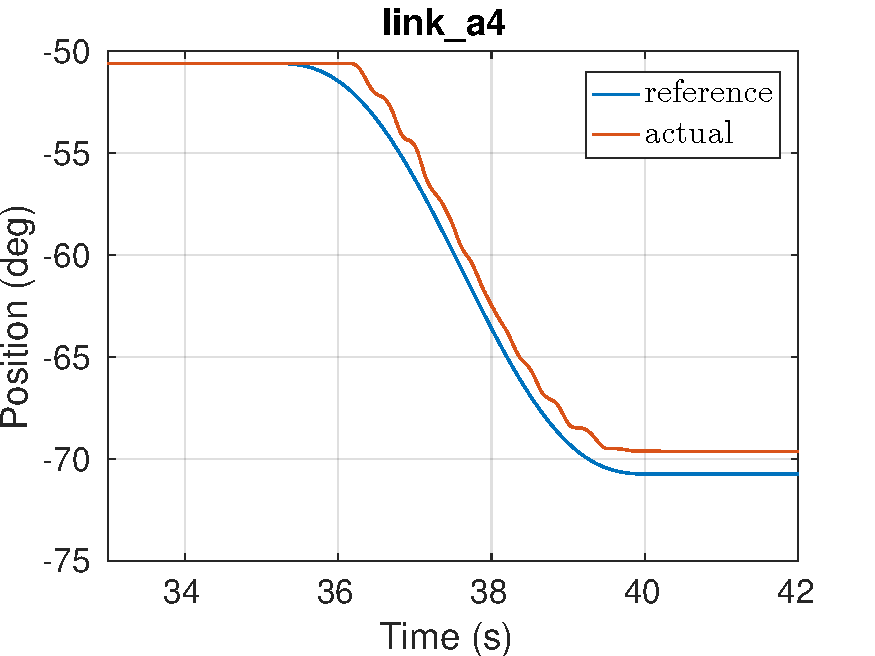
\includegraphics[scale=0.34]{cart_real_3_a4} &
      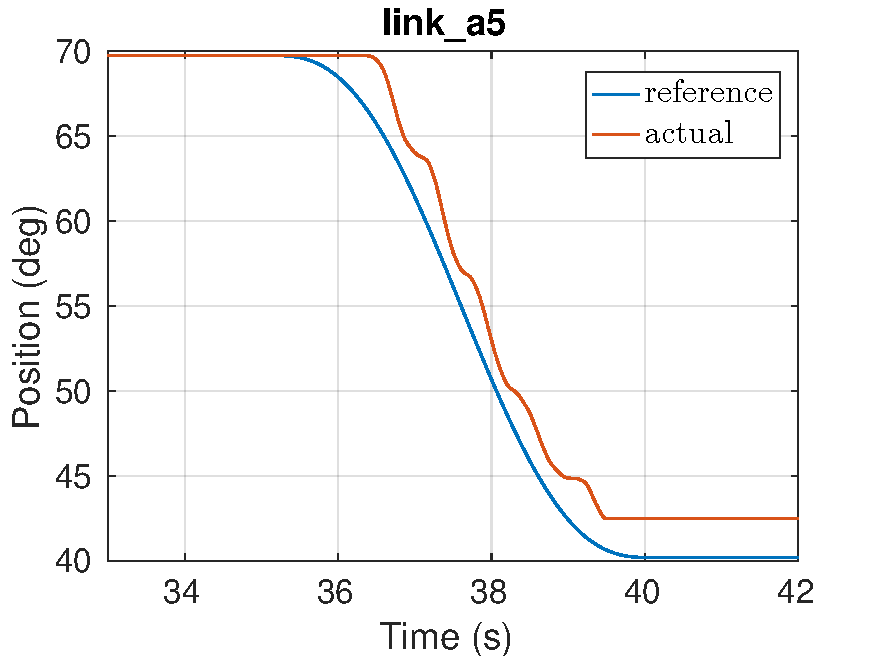
\includegraphics[scale=0.34]{cart_real_3_a5}
    \end{tabular}
  \end{center}
  \begin{center}
   \vskip-0.1in
    \begin{tabular}{c}
      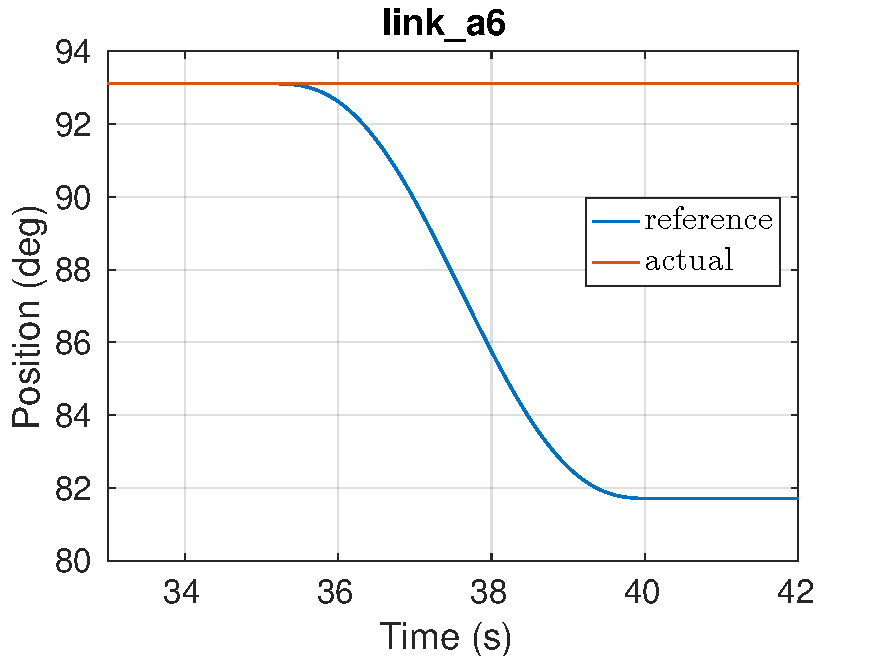
\includegraphics[scale=0.34]{cart_real_3_a6}
    \end{tabular}
  \end{center}
\end{frame}

\begin{frame}
  \frametitle{Experimental setup}
  \framesubtitle{Force regulation}
  \begin{itemize}
  \item[-] duration $2$s
  \item[-] $K_p = \mathrm{diag}(300)$
  \item[-] $K_d = \mathrm{diag}(30)$
  \item[-] $b_f = 25$
  \end{itemize}
\end{frame}

\begin{frame}
  \frametitle{Experimental setup}
  \framesubtitle{Force regulation - Results ($k_{f} = 1$)}
  \begin{center}
   \vskip-0.1in
    \begin{tabular}{ccc}
      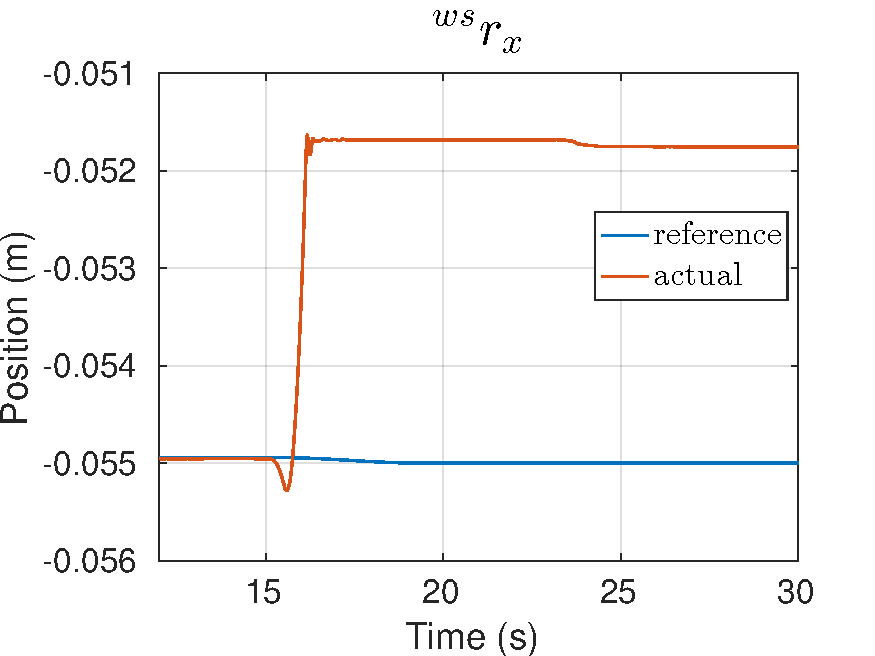
\includegraphics[scale=0.26]{force_real_13_x} &
      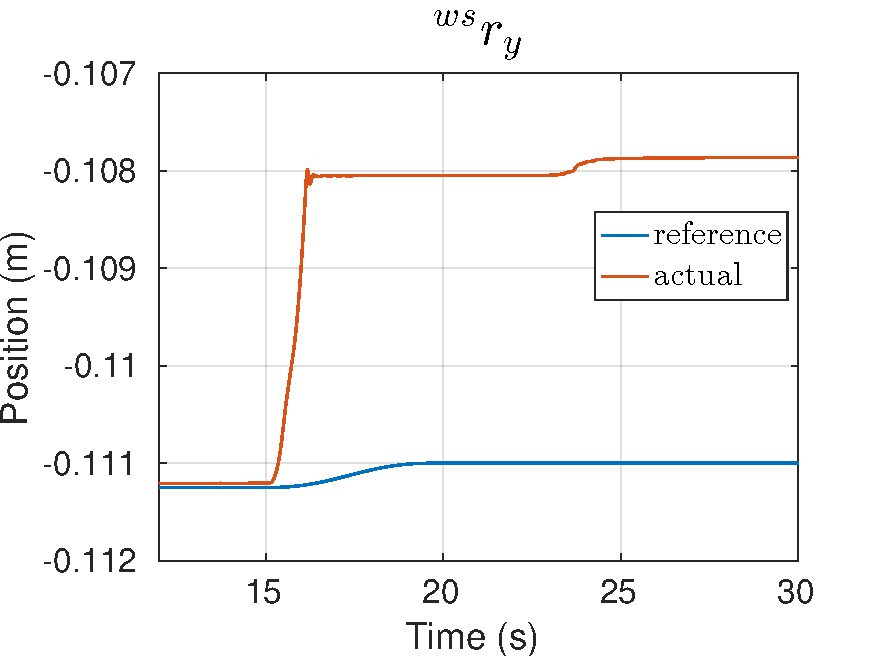
\includegraphics[scale=0.26]{force_real_13_y} &
      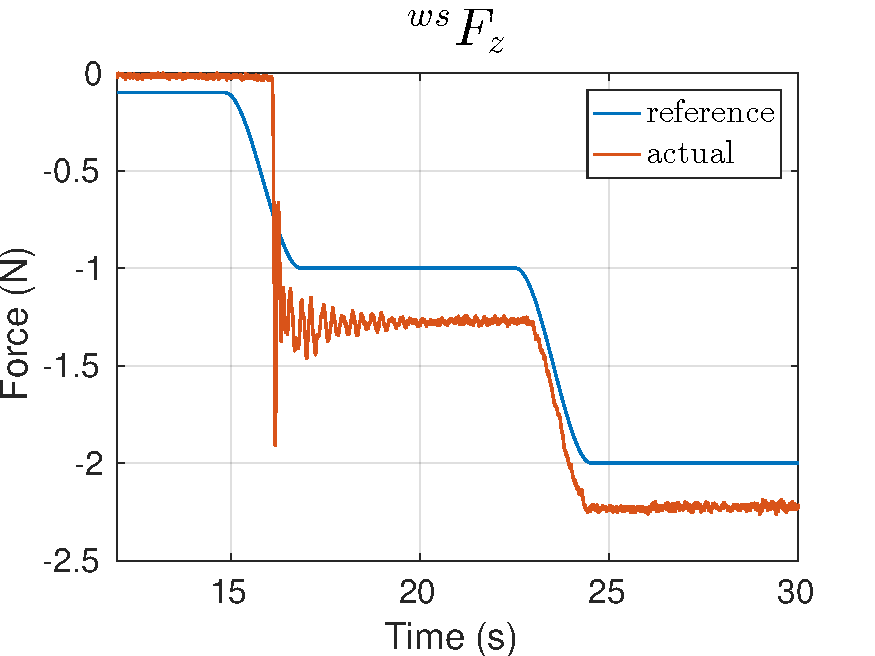
\includegraphics[scale=0.26]{force_real_13_z} \\
      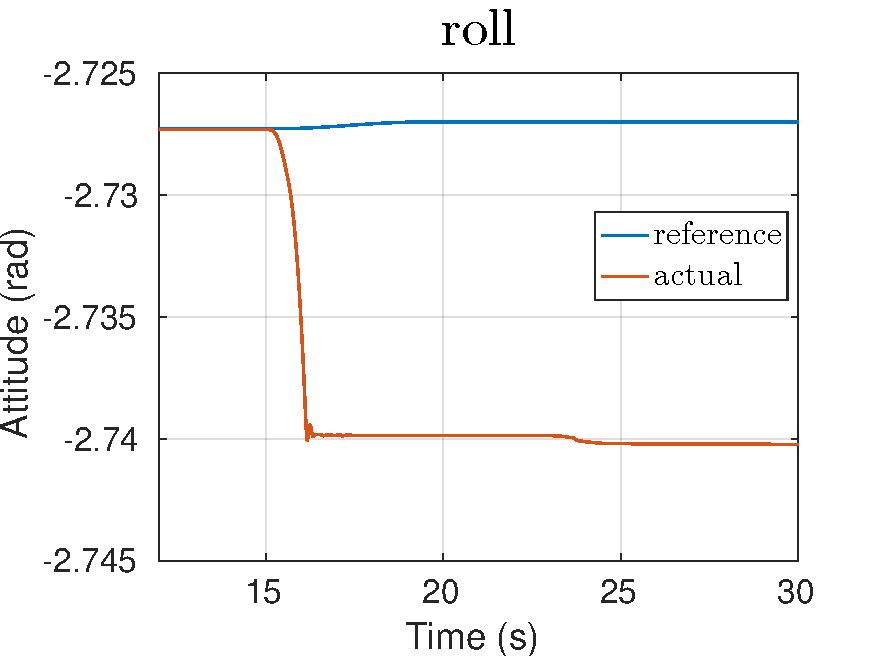
\includegraphics[scale=0.26]{force_real_13_roll} &
      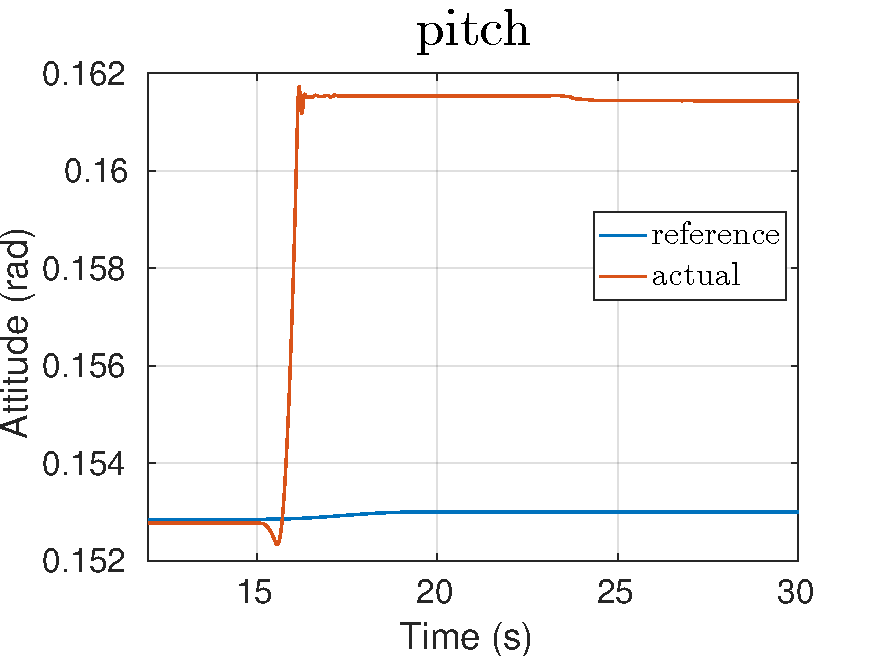
\includegraphics[scale=0.26]{force_real_13_pitch} &
      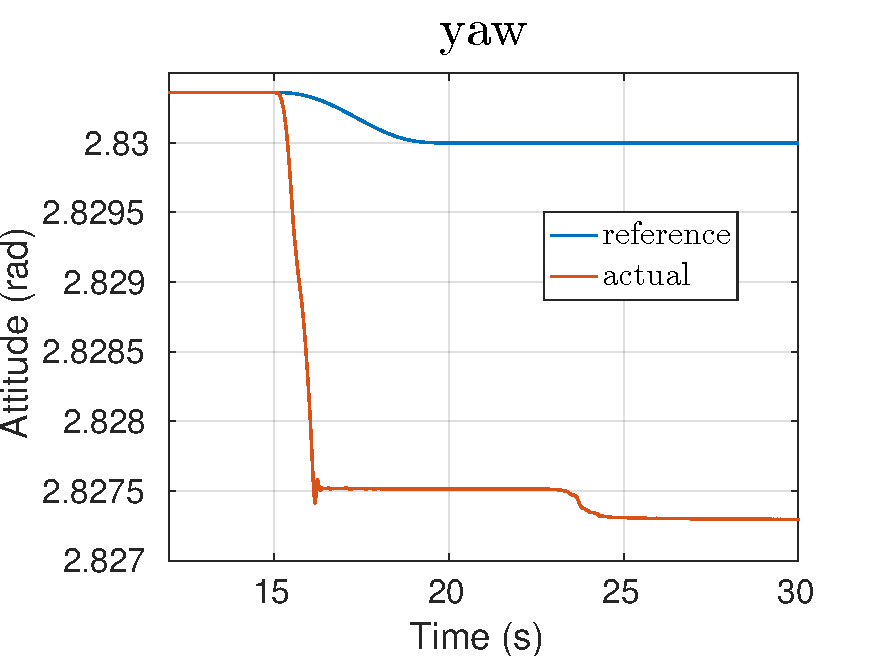
\includegraphics[scale=0.26]{force_real_13_yaw}
    \end{tabular}
  \end{center}
\end{frame}

\begin{frame}
  \frametitle{Experimental setup}
  \framesubtitle{Force regulation - Results ($k_{f} = 1.5$)}
  \begin{center}
   \vskip-0.1in
    \begin{tabular}{ccc}
      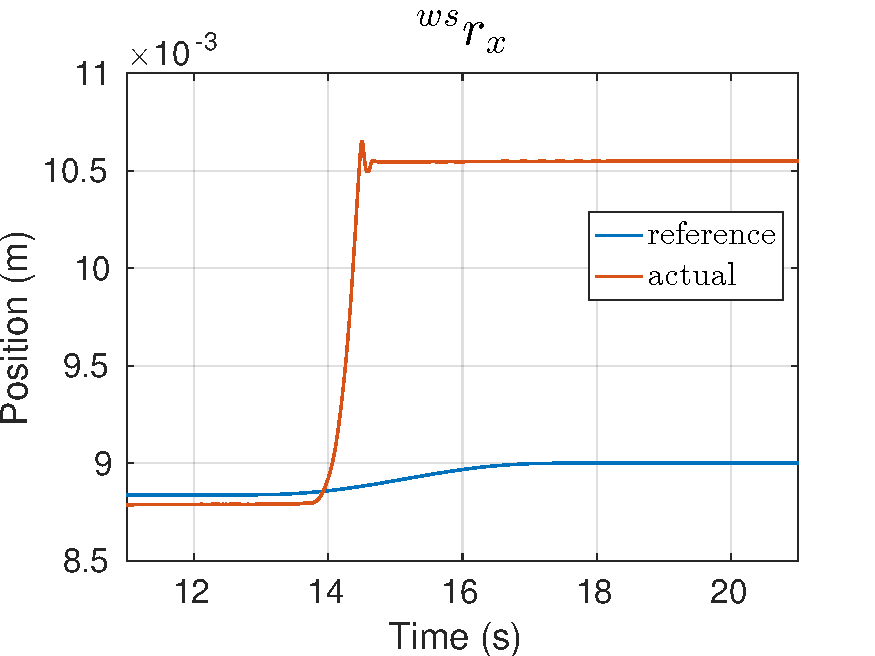
\includegraphics[scale=0.26]{force_real_16_x} &
      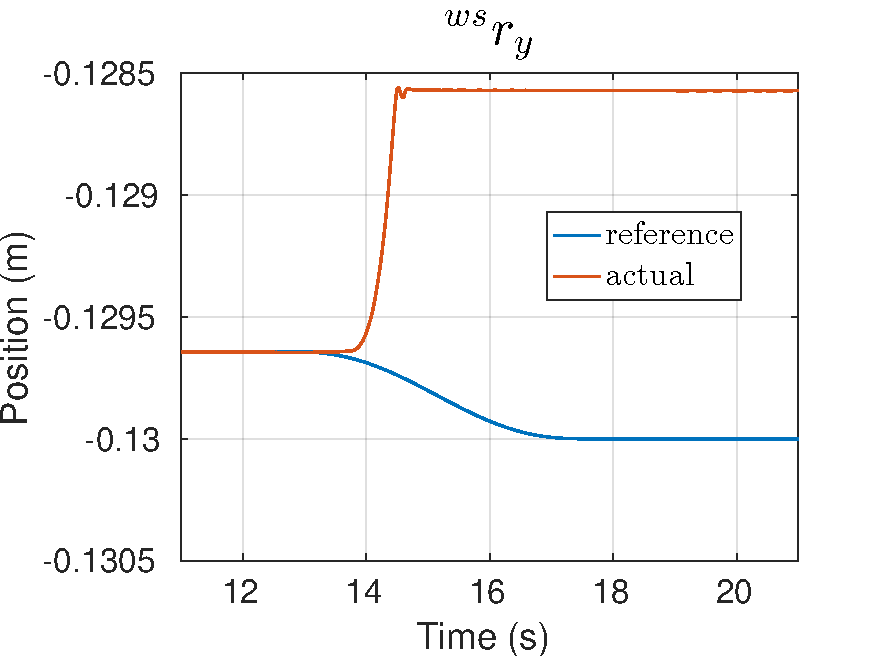
\includegraphics[scale=0.26]{force_real_16_y} &
      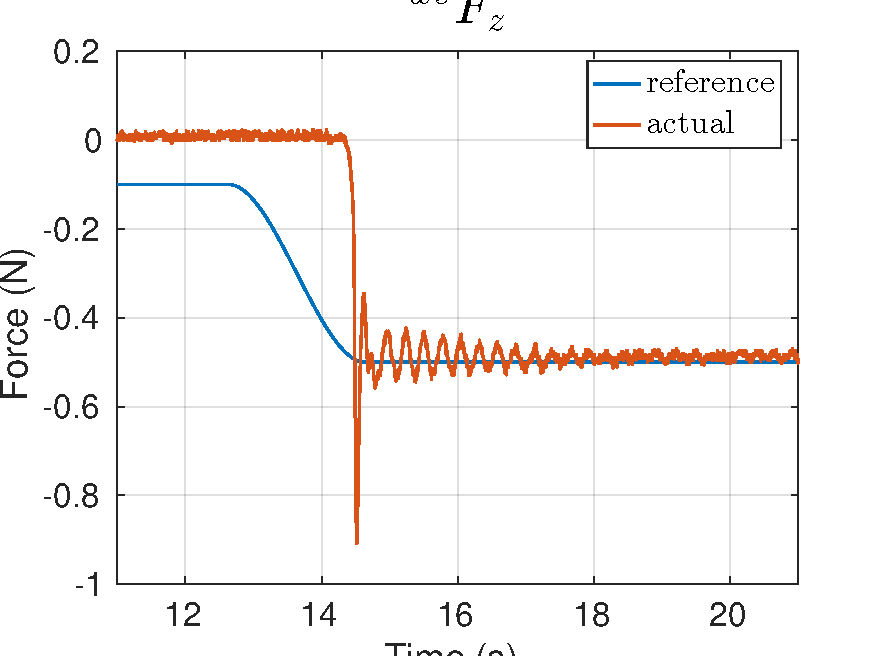
\includegraphics[scale=0.26]{force_real_16_z} \\
      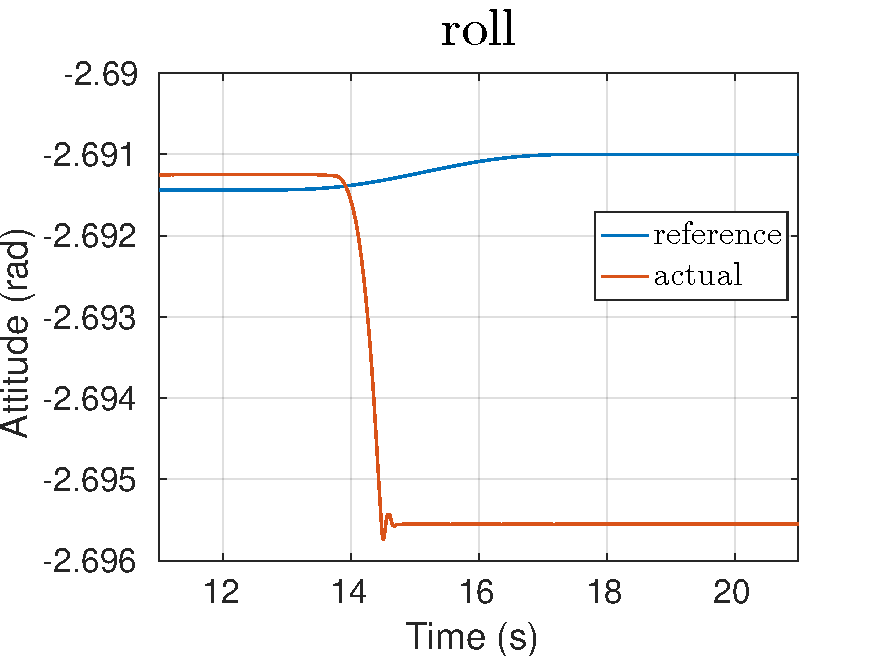
\includegraphics[scale=0.26]{force_real_16_roll} &
      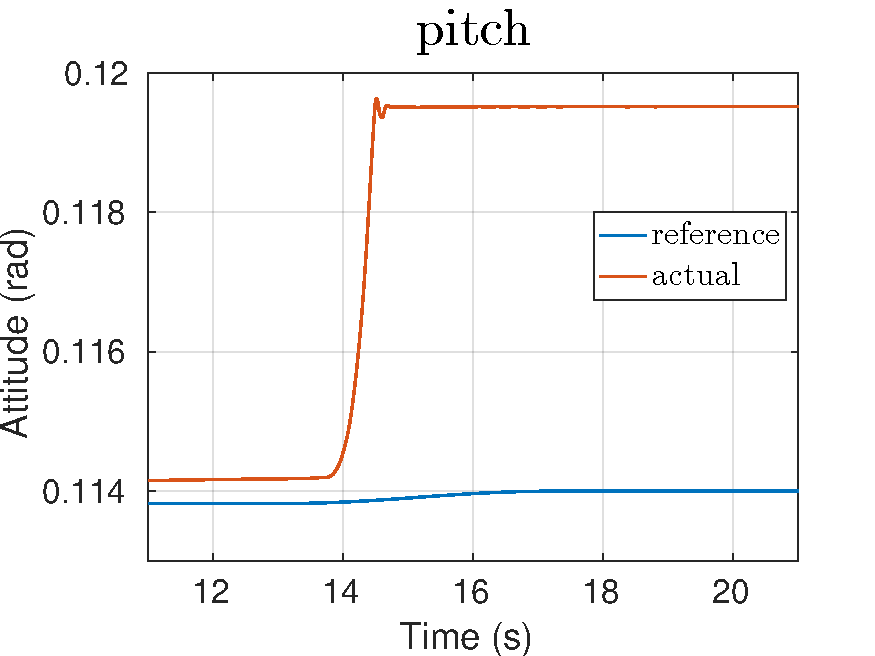
\includegraphics[scale=0.26]{force_real_16_pitch} &
      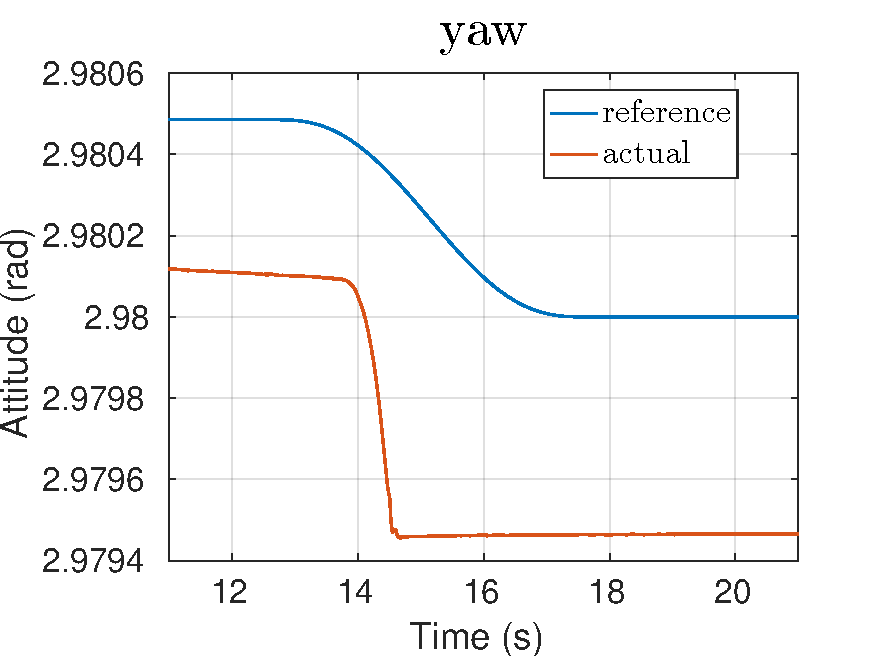
\includegraphics[scale=0.26]{force_real_16_yaw}
    \end{tabular}
  \end{center}
\end{frame}

\begin{frame}
  \frametitle{Experimental setup}
  \framesubtitle{Force regulation + motion}
  \begin{itemize}
  \item[-] reference trajectory duration $5$s
  \item[-] reference force duration $2$s
  \item[-] $K_p = \mathrm{diag}(300)$
  \item[-] $K_d = \mathrm{diag}(30)$
  \item[-] $k_{f} = 1.5$
  \item[-] $b_f = 25$
  \end{itemize}
\end{frame}

\begin{frame}
  \frametitle{Experimental setup}
  \framesubtitle{Force regulation + motion - Results}
  \begin{center}
   \vskip-0.1in
    \begin{tabular}{ccc}
      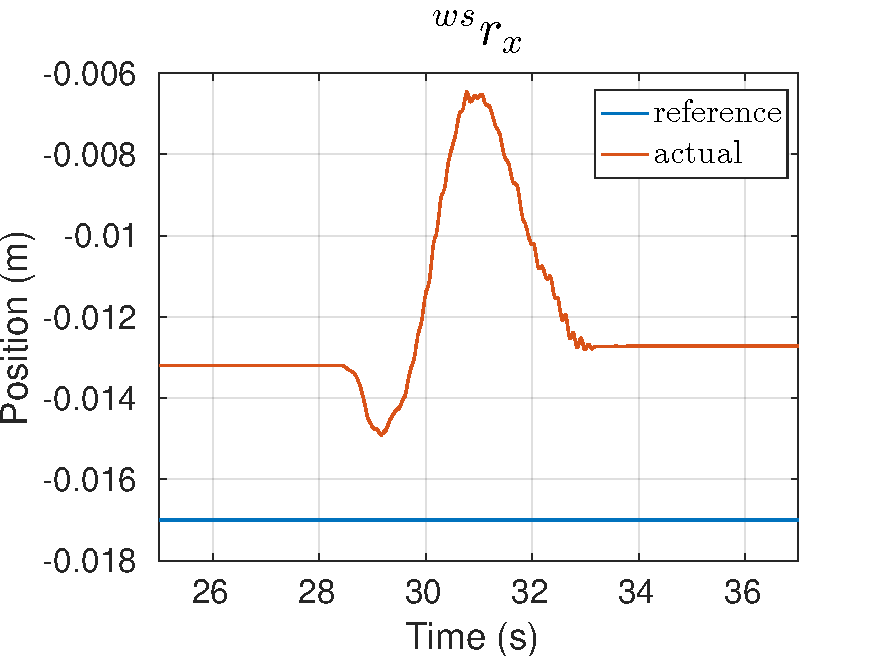
\includegraphics[scale=0.26]{force_real_11_x} &
      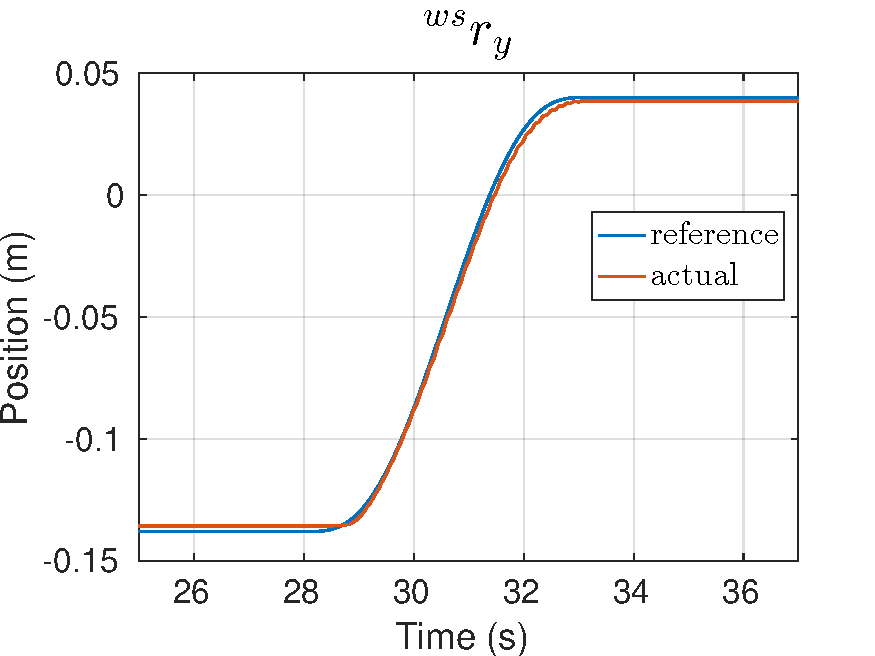
\includegraphics[scale=0.26]{force_real_11_y} &
      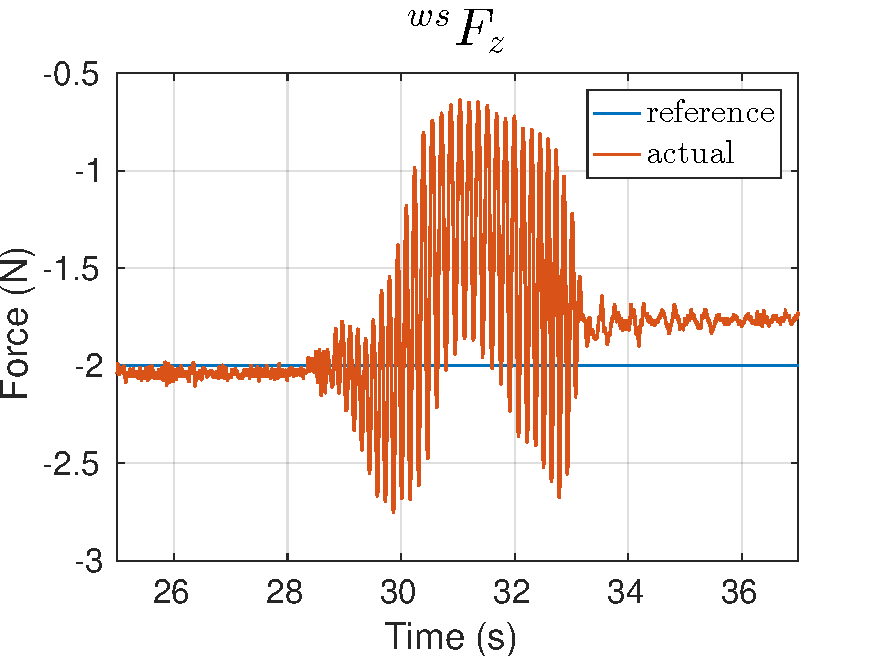
\includegraphics[scale=0.26]{force_real_11_z} \\
      \includegraphics[scale=0.26]{force_real_11_roll} &
      \includegraphics[scale=0.26]{force_real_11_pitch} &
      \includegraphics[scale=0.26]{force_real_11_yaw}
    \end{tabular}
  \end{center}
\end{frame}

\begin{frame}
  \frametitle{Experimental setup}
  \framesubtitle{Force regulation + motion - Results}
  \begin{center}
   \vskip-0.1in
    \begin{tabular}{ccc}
      \includegraphics[scale=0.26]{force_real_10_x} &
      \includegraphics[scale=0.26]{force_real_10_y} &
      \includegraphics[scale=0.26]{force_real_10_z} \\
      \includegraphics[scale=0.26]{force_real_10_roll} &
      \includegraphics[scale=0.26]{force_real_10_pitch} &
      \includegraphics[scale=0.26]{force_real_10_yaw}
    \end{tabular}
  \end{center}
\end{frame}

\section{Software implementation}
\begin{frame}{Some notes about implementation}
  \begin{itemize}
  \item[-] ROS based software
  \item[-] already existing (Centro Piaggio) KUKA LWR4+ software stack (model, FRI, F/T sensor interface, ROS controllers)
  \item[-] built upon KinematicChainControllerBase (KDL facilities)
  \item[-] extends KinematicChainControllerBase by providing an Operational Space Inverse Dynamics \emph{abstract} controller
    \begin{itemize}
    \item[-] arbitrary commanded acceleration in operational space
    \item[-] state (with derivatives) ready to use and projected in $ws$
    \item[-] jacobian extended to take into account the length of the tool
    \item[-] null projection available
    \end{itemize}
  \item[-] Hybrid Impedance Controller based on Inverse Dynamics Controller
  \end{itemize}
\end{frame}

\end{document}
